  % this file is called up by thesis.tex
% content in this file will be fed into the main document
% ----------------------- name of chapter  -------------------------
\newgeometry{top=-0.9cm, left=1.2cm, right=1.5cm, bottom=1.45cm}
\chapter{Signal + Background fit in SRs+CRs using SMT}
\label{app:stat_smt:tzc:splusb:crsr}
% ----------------------- paths to graphics ------------------------

% change according to folder and file names
\ifpdf
\graphicspath{Appendices/AP8/figures/SPLUSB_CRSR_UsingSMTFullSys}
\else
\graphicspath{Appendices/AP8/figures/SPLUSB_CRSR_UsingSMTFullSys}
\fi
\vspace{-1cm}
To extract the expected sensitivity, an SRs+CRs S+B fit is performed. 
Real data in used in CRs while in SRs an Asimov dataset is used,
constructed using the background normalisations as done in Appendix \ref{app:stat:tzc:bonly:cr} for the selection using \DLrc.\\
A summary of plots and tables shown in this section are the following:
\begin{itemize}
	\item The value of the post-fit normalisation parameters of the free floating background is shown in \Cref{fig:stat_smt:tzc:splusb:crsr:norm}.
	\item The pull distributions of the all nuisance parameters can be seen in \Cref{fig:stat_smt:tzc:splusb:crsr:np:instr,fig:stat_smt:tzc:splusb:crsr:np:model} and \Cref{fig:stat_smt:tzc:splusb:crsr:gamma}. 
	\item The correlation matrix of the nuisance parameters is shown in \Cref{fig:stat_smt:tzc:splusb:crsr:corrmatrix}. 
	\item The list of the systematic shapes that are dropped from the fit for each sample and for each region is shown in \Cref{fig:stat_smt:tzc:splusb:crsr:pruning}.
	\item The ranking of the nuisance parameters is shown in \Cref{fig:stat_smt:tzc:splusb:crsr:ranking}. 
	%Red and blue plots for the top five ranked NPs are shown in a
	%dedicated appendix (\Cref{sec:app:fit:redblue:tzc:splusb:crsr}).\\
	\item Event yields pre- and post-fit are shown in \Cref{tab:stat_smt:tzc:splusb:crsr:yields:prefit,tab:stat_smt:tzc:splusb:crsr:yields:postfit}. 
	\item Pre-fit and post-fit distributions of the fitted distributions in the various regions are shown in \Cref{fig:stat_smt:tzc:splusb:crsr:srplots:1,fig:stat_smt:tzc:splusb:crsr:srplots:2,fig:stat_smt:tzc:splusb:crsr:crplots:1,fig:stat_smt:tzc:splusb:crsr:crplots:2}.
	\item Expected limits on the branching ratios of $\Pqt\rightarrow\PZ\Pqc$ shown in \Cref{tab:results:limits_smt}.
\end{itemize}
Normalisation factors (\cref{fig:stat_smt:tzc:splusb:crsr:norm}) and NP
pulls and constrains 
(\Cref{fig:stat_smt:tzc:splusb:crsr:np:instr,fig:stat_smt:tzc:splusb:crsr:np:model}) 
are very similar. 
%The most pulled NPs (e.g. \ttbar FSR, \VVHF 
%normalisation, and \VVHF Berends scaling for events with 1 jet) are
%not among the highest ranked NPs
%(\Cref{fig:stat_smt:tzc:splusb:crsr:ranking}). 
%Slightly pulled NPs (e.g. Other fakes norm. and \ttZ norm.) have a small impact on the signal strength, around 2\%.\\
None of the systematic uncertainties has a post-fit impact on the signal strength parameter greater than 4\%.
Concerning the correlations between NPs
(\Cref{fig:stat_smt:tzc:splusb:crsr:corrmatrix}), some strong correlations
between diboson related NPs are present, as expected. This is also
true for the \ttbar normalisation and some \ttbar modeling NPs. 

\begin{figure}[htbp]
	\centering
	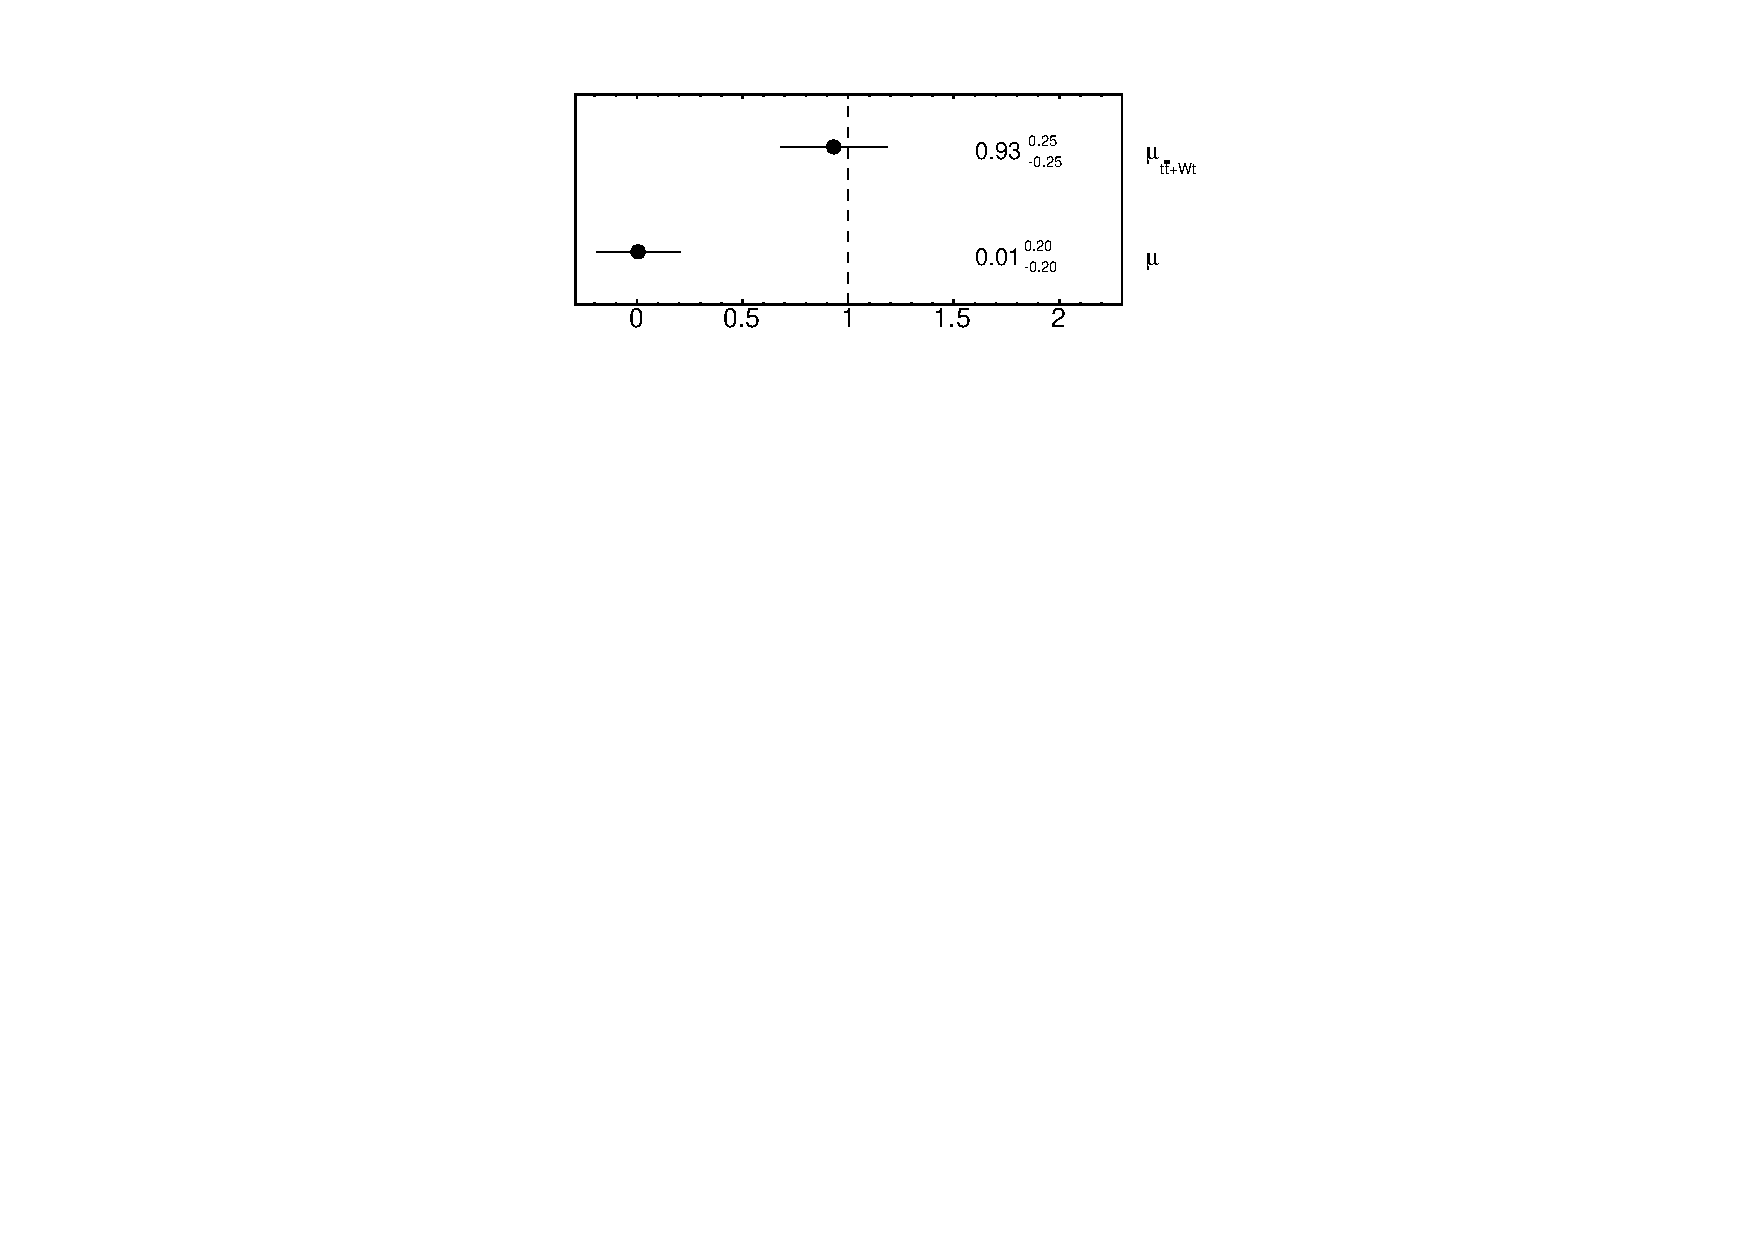
\includegraphics[width=.42\textwidth]{Appendices/AP8/figures/SPLUSB_CRSR_UsingSMTFullSys/NormFactors}
	\caption{Normalisation factors for the S+B \tZc fit in SRs+CRs with realistic Asimov.}%
	\label{fig:stat_smt:tzc:splusb:crsr:norm}
\end{figure}
\restoregeometry

\begin{figure}[htbp]
	\centering
	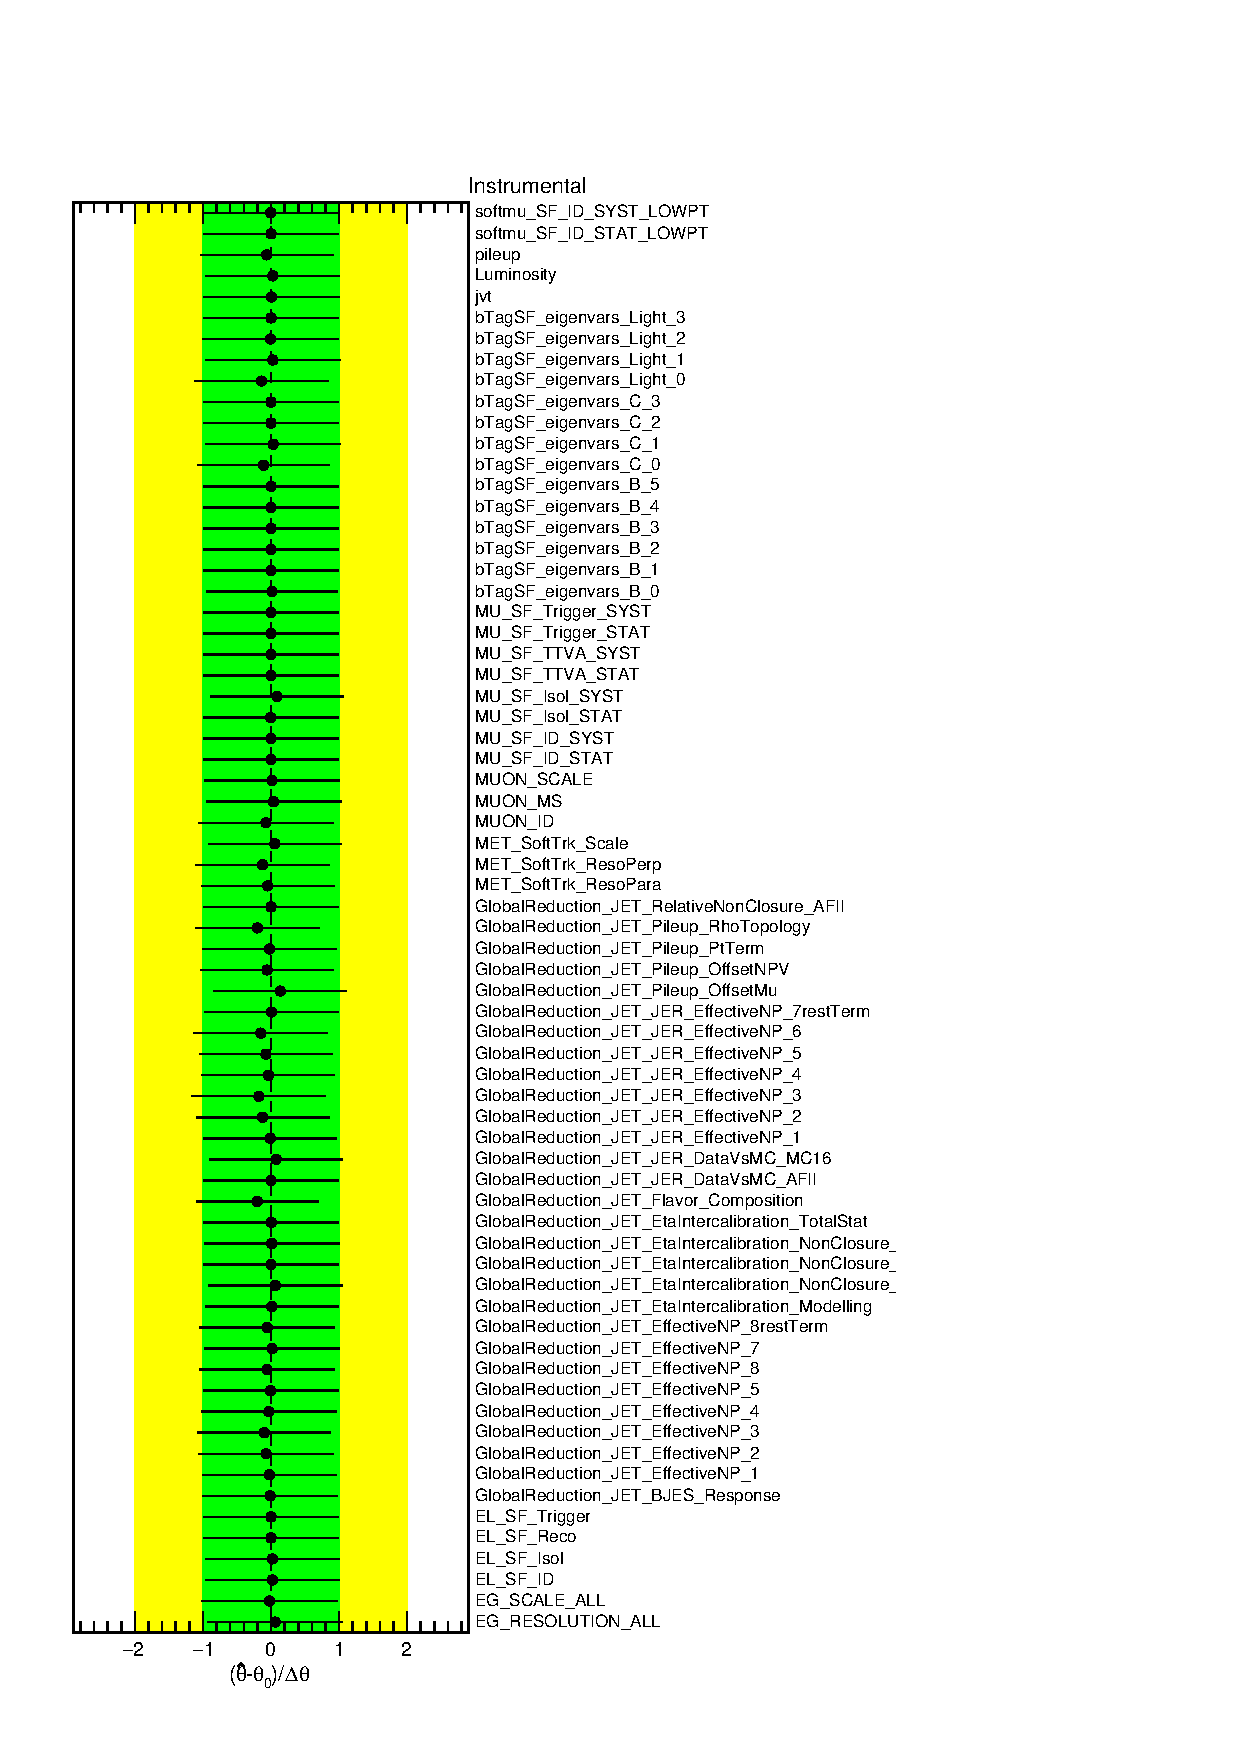
\includegraphics[width=.8\textwidth]{Appendices/AP8/figures/SPLUSB_CRSR_UsingSMTFullSys/NuisPar_Instrumental}
	\caption{Pulls and constraints of the instrumental nuisance parameters for the S+B \tZc fit in SRs+CRs with realistic Asimov.}%
	\label{fig:stat_smt:tzc:splusb:crsr:np:instr}
\end{figure}

\begin{figure}[htbp]
	\centering
	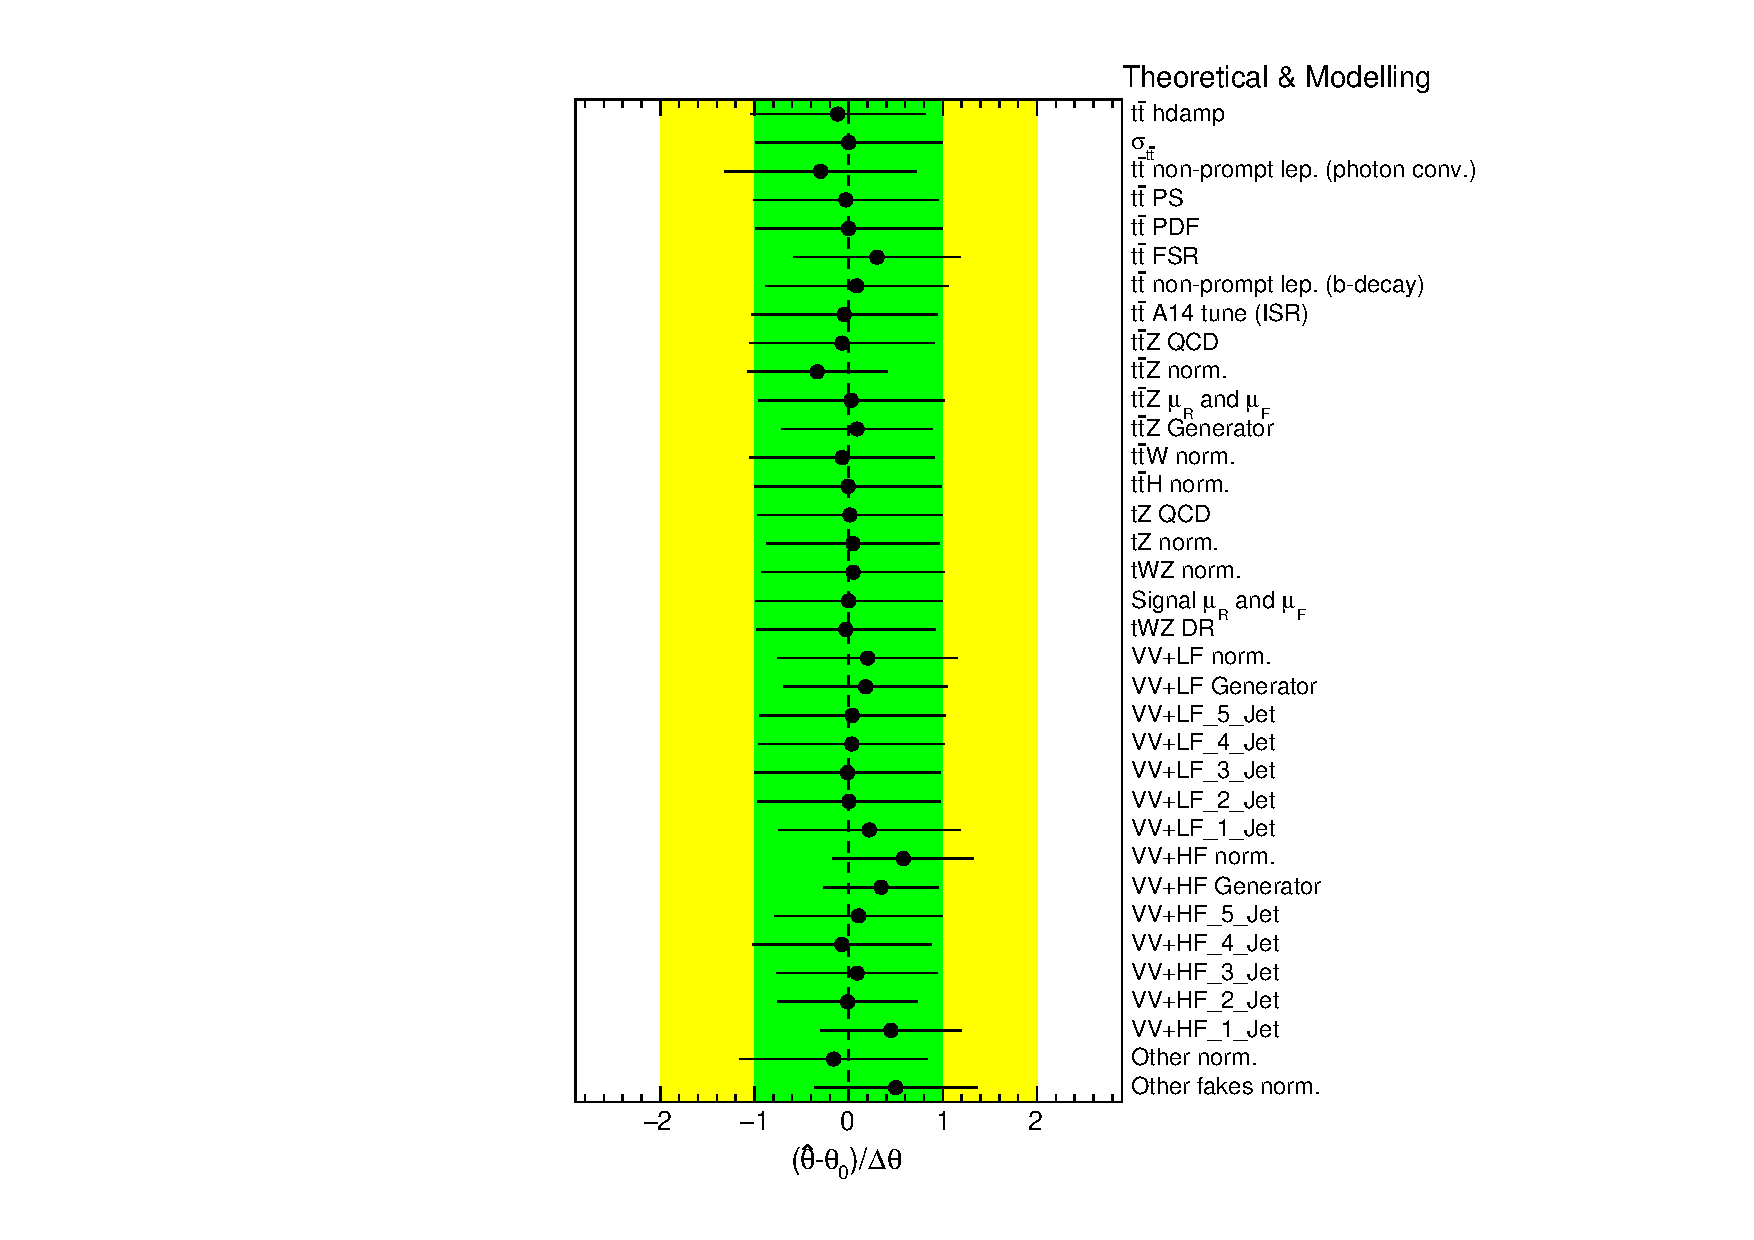
\includegraphics[width=.85\textwidth]{Appendices/AP8/figures/SPLUSB_CRSR_UsingSMTFullSys/NuisPar_Theoretical_&_Modelling}
	\caption{Pulls and constraints of the theoretical and modeling nuisance parameters for the S+B \tZc fit in SRs+CRs with realistic Asimov.}%
	\label{fig:stat_smt:tzc:splusb:crsr:np:model}
\end{figure}

\begin{figure}[htbp]
	\centering
	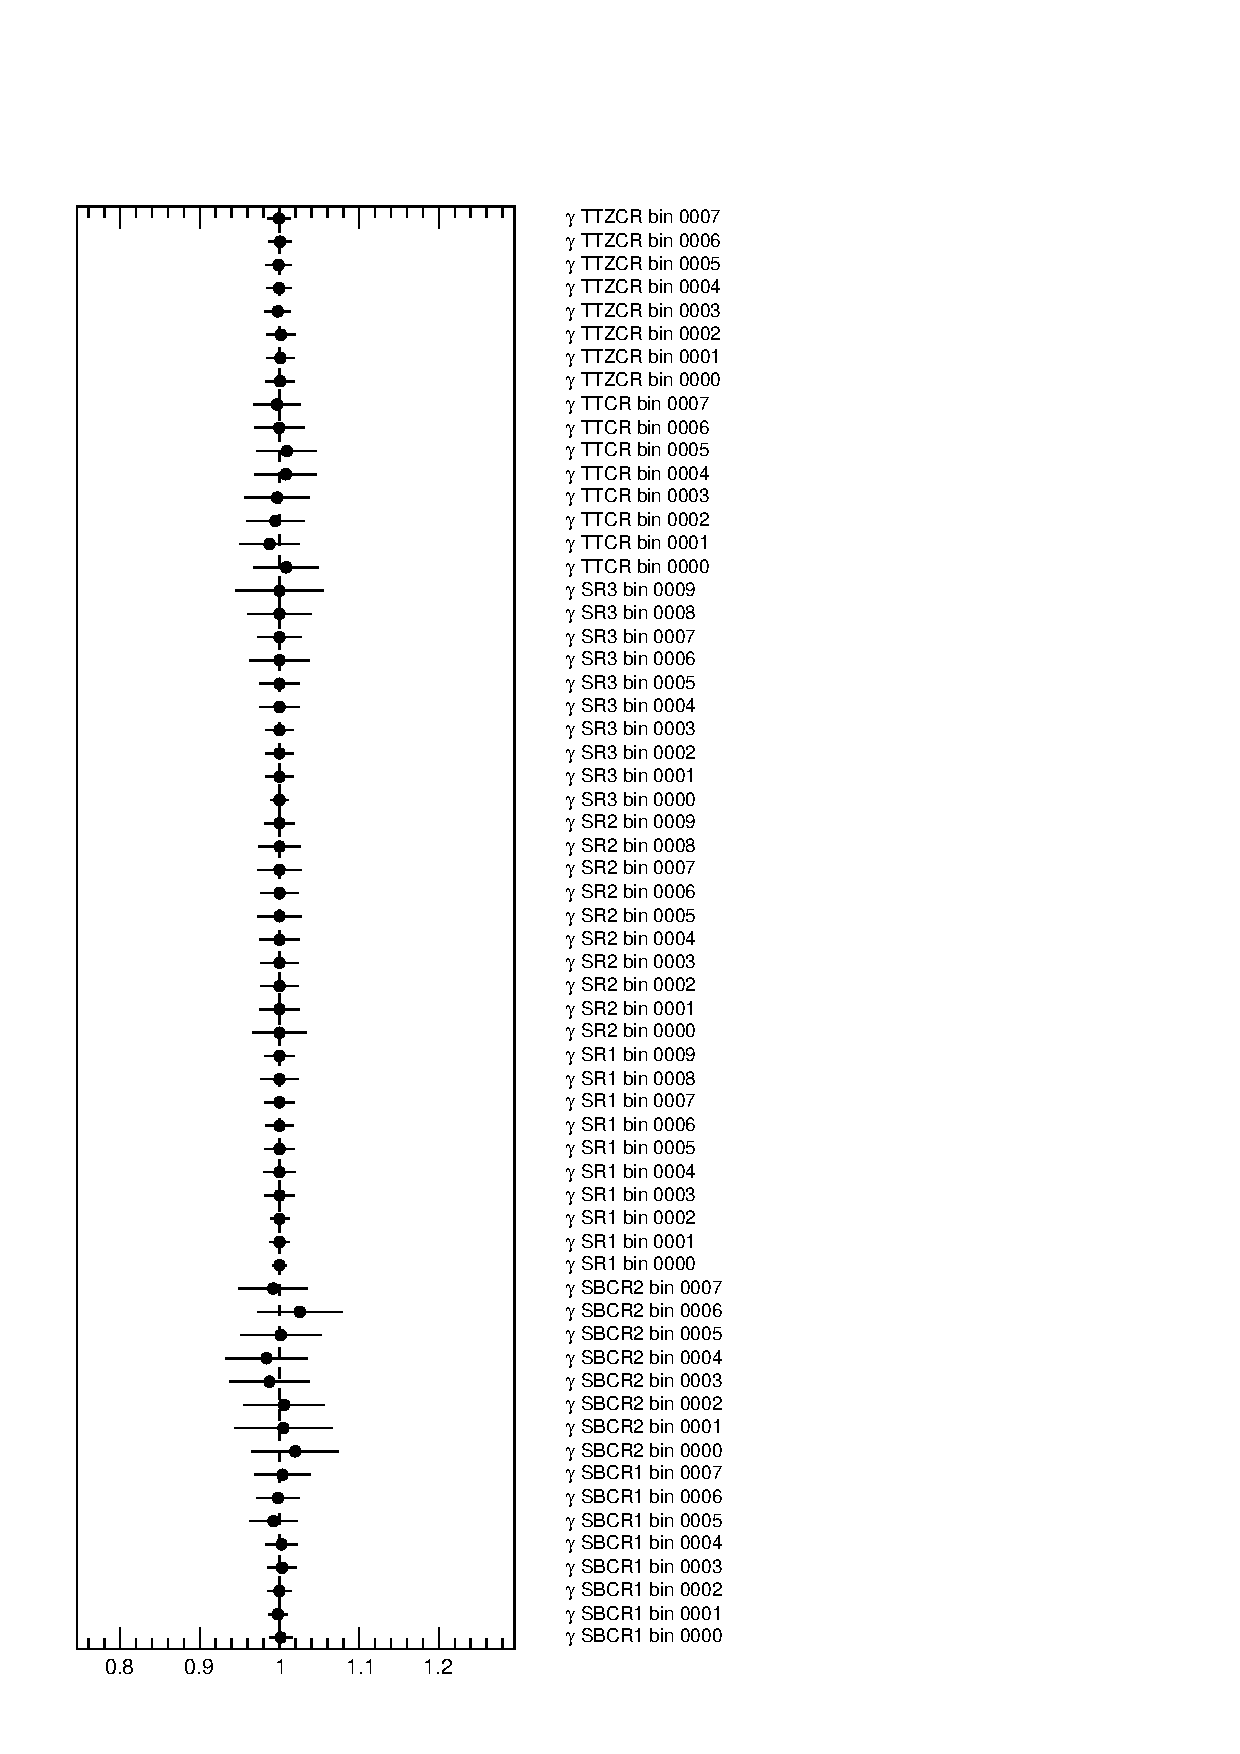
\includegraphics[width=.85\textwidth]{Appendices/AP8/figures/SPLUSB_CRSR_UsingSMTFullSys/Gammas}
	\caption{Gamma parameters for the S+B \tZc fit in SRs+CRs with realistic Asimov.}%
	\label{fig:stat_smt:tzc:splusb:crsr:gamma}
\end{figure}

\begin{figure}[htbp]
	\centering
	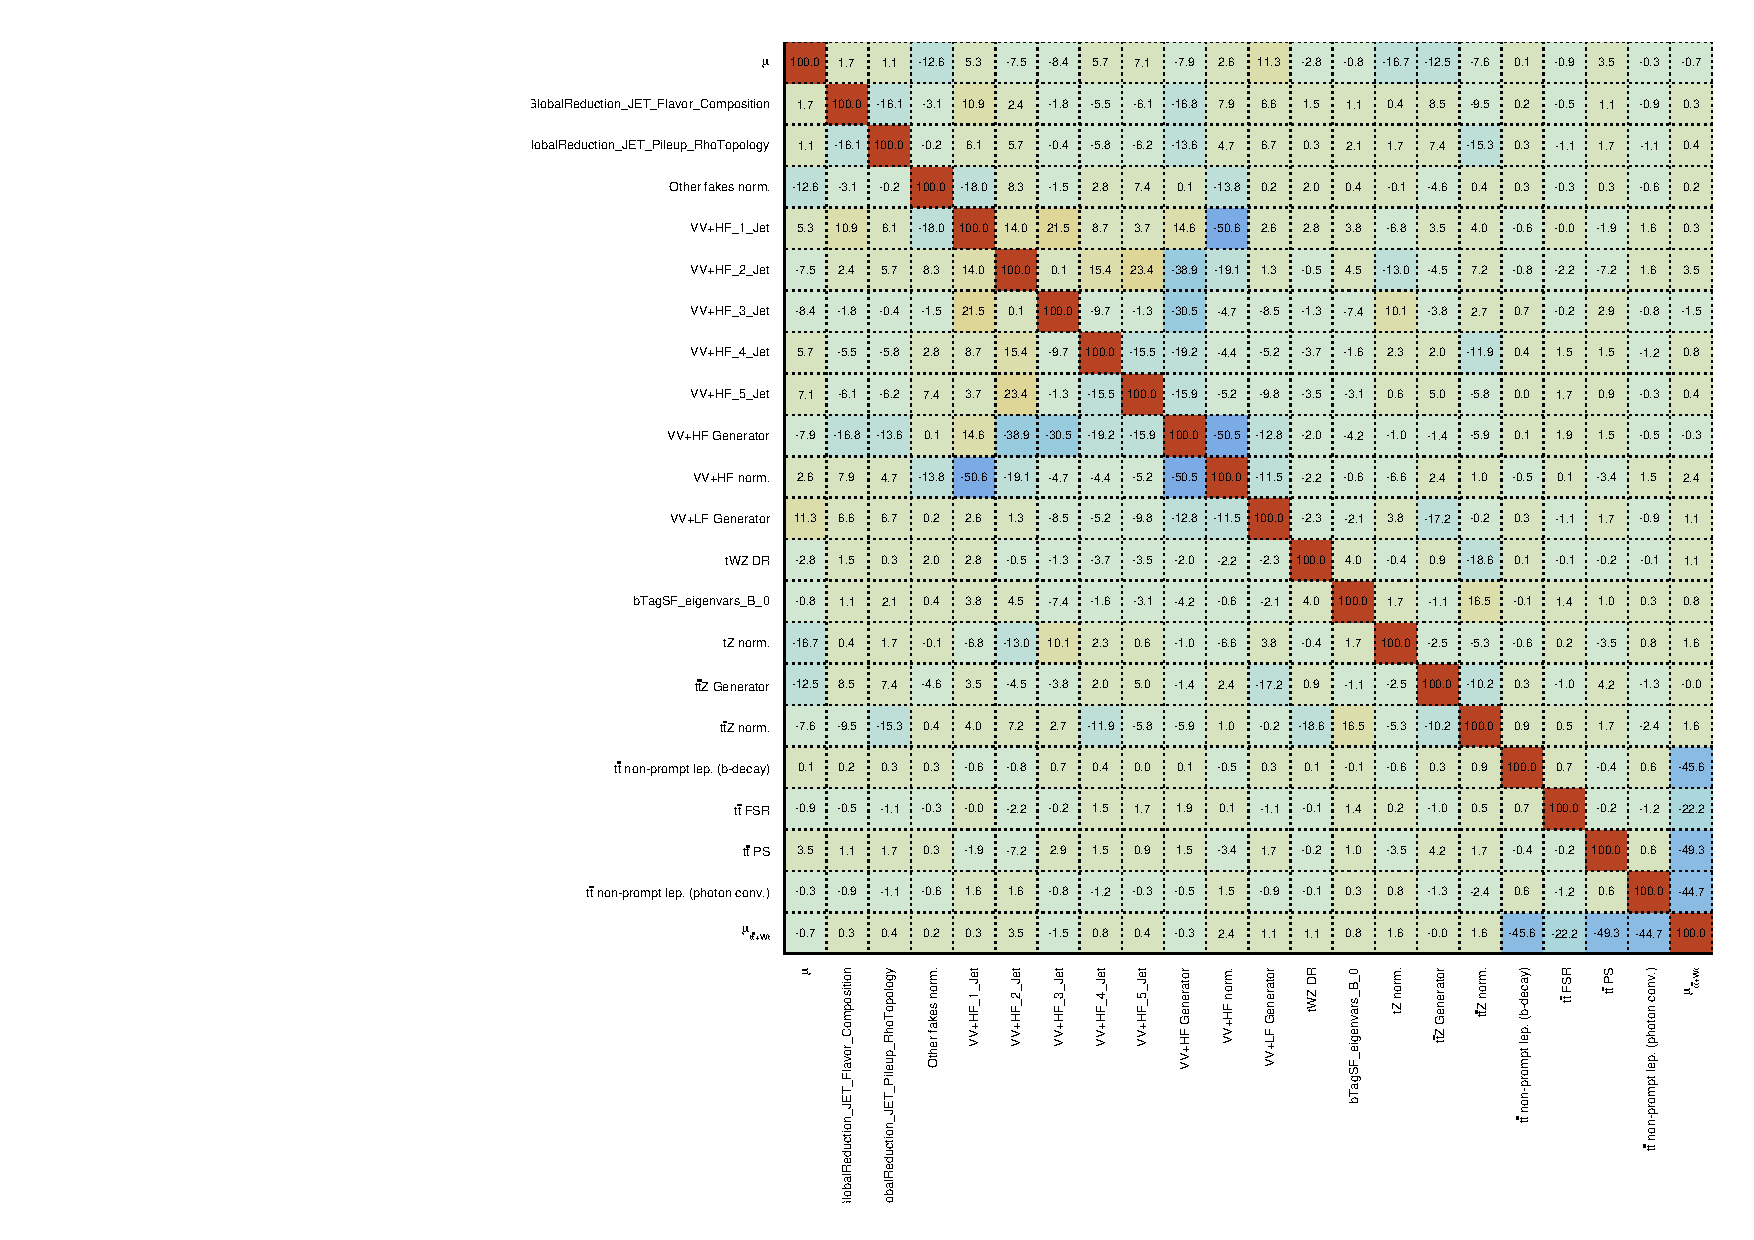
\includegraphics[width=.95\textwidth]{Appendices/AP8/figures/SPLUSB_CRSR_UsingSMTFullSys/CorrMatrix}
	\caption{Correlation matrix of the nuisance paramenters for the S+B \tZc fit in SRs+CRs with realistic Asimov.}%
	\label{fig:stat_smt:tzc:splusb:crsr:corrmatrix}
\end{figure}

\begin{figure}[htbp]
	\centering
	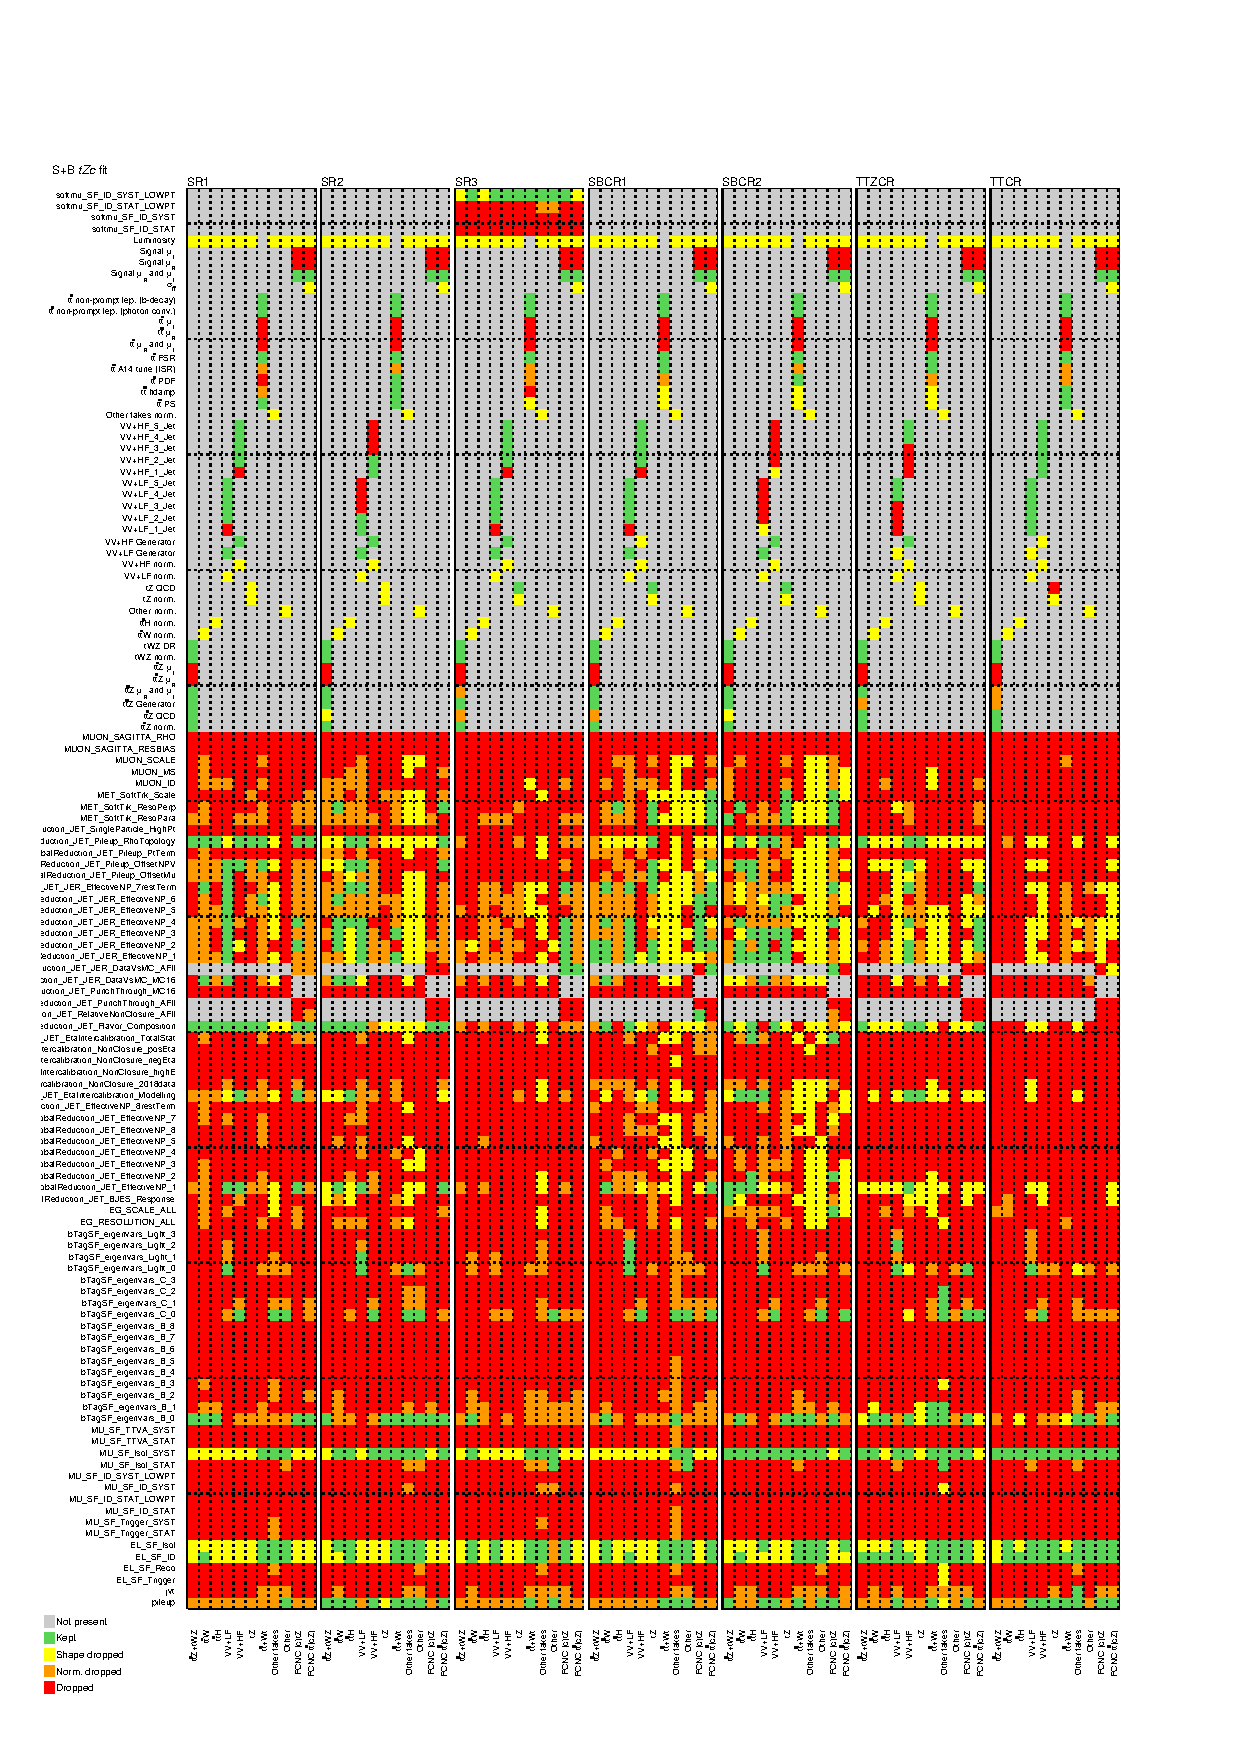
\includegraphics[width=.85\textwidth]{Appendices/AP8/figures/SPLUSB_CRSR_UsingSMTFullSys/Pruning}
	\caption{Pruning of the nuisance parameters for the S+B \tZc fit in SRs+CRs with realistic Asimov.}%
	\label{fig:stat_smt:tzc:splusb:crsr:pruning}
\end{figure}

\begin{figure}[htbp]
	\centering
	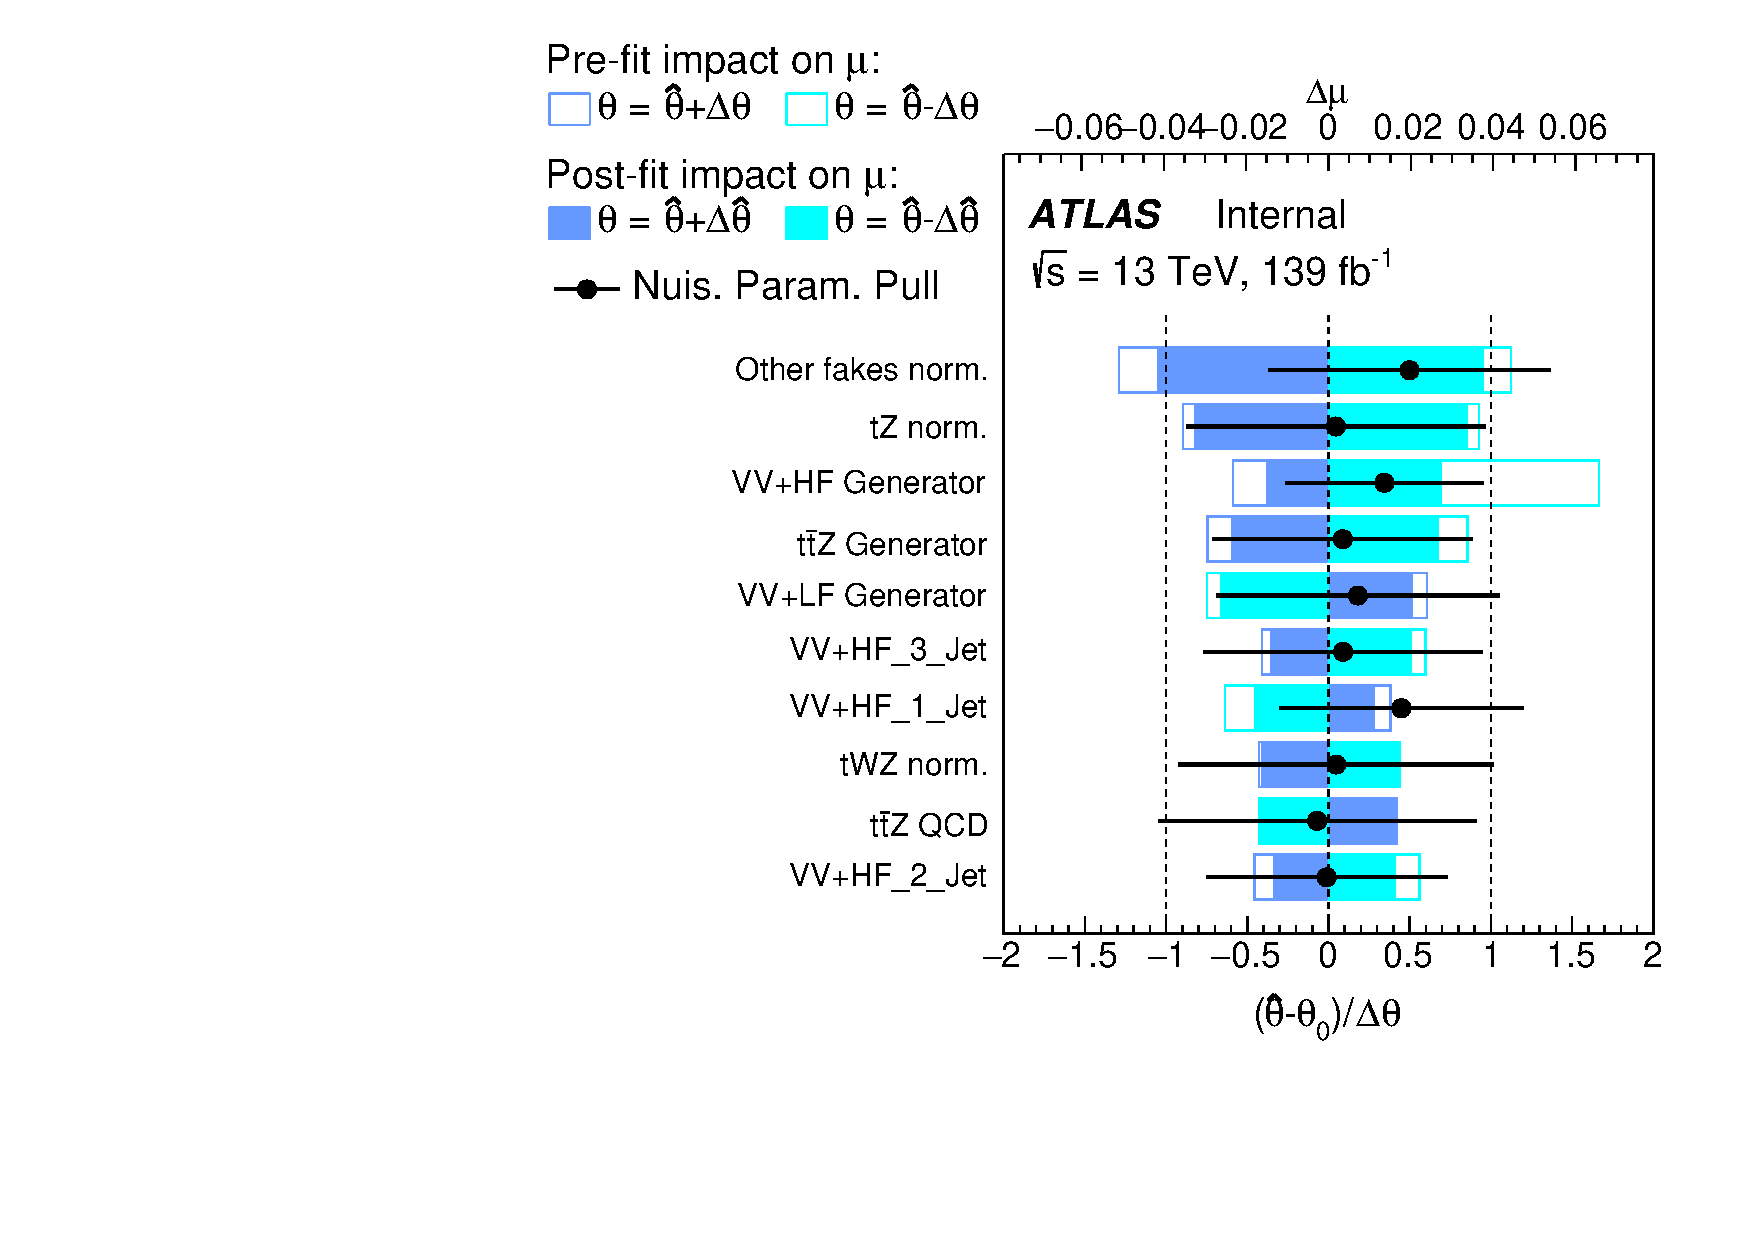
\includegraphics[width=.9\textwidth]{Appendices/AP8/figures/SPLUSB_CRSR_UsingSMTFullSys/Ranking}
	\caption{Ranking of the nuisance parameters for the S+B \tZc fit in SRs+CRs with realistic Asimov.}%
	\label{fig:stat_smt:tzc:splusb:crsr:ranking}
\end{figure}

\FloatBarrier
\clearpage
%\global\pdfpageattr\expandafter{\the\pdfpageattr/Rotate 90}
\begin{table}[]
	\centering
	\tiny
	% NB: add to main document: 
% \usepackage{siunitx} 
% \sisetup{separate-uncertainty,table-format=6.3(6)}  % hint: modify table-format to best fit your tables
\begin{tabular}{|p{0.10\textwidth}|>{\centering}p{0.08\textwidth}|>{\centering}p{0.08\textwidth}|>{\centering}p{0.08\textwidth}|>{\centering}p{0.09\textwidth}|>{\centering}p{0.09\textwidth}|>{\centering}p{0.09\textwidth}|>{\centering\arraybackslash}p{0.09\textwidth}|}
\toprule  
 & {SR1tZc} & {SR2tZc} & {SR3tZc} & {Side-band CR1} & {Side-band CR2} & {\ttZ CR} & {\ttbar CR}\\
\midrule 
\ttZ+\tWZ   & 200 $\pm$ 26 & 36 $\pm$ 7 & 97 $\pm$ 22 & 88 $\pm$ 12 & 9.1 $\pm$ 2.1 & 164 $\pm$ 22 & 14.8 $\pm$ 1.9 \\ 
\ttW   & 6.5 $\pm$ 1.1 & 3.5 $\pm$ 0.6 & 2.5 $\pm$ 0.4 & 4.3 $\pm$ 0.7 & 2.5 $\pm$ 0.5 & 2.3 $\pm$ 0.4 & 27 $\pm$ 4 \\ 
\ttH   & 7.4 $\pm$ 1.2 & 0.93 $\pm$ 0.18 & 3.1 $\pm$ 0.5 & 2.3 $\pm$ 0.4 & 0.36 $\pm$ 0.07 & 5.4 $\pm$ 0.9 & 13.8 $\pm$ 2.1 \\ 
\VVLF   & 29 $\pm$ 18 & 35 $\pm$ 13 & 36 $\pm$ 20 & 25 $\pm$ 15 & 18 $\pm$ 7 & 0.20 $\pm$ 0.22 & 0.40 $\pm$ 0.20 \\ 
\VVHF   & 150 $\pm$ 110 & 160 $\pm$ 70 & 80 $\pm$ 50 & 130 $\pm$ 80 & 69 $\pm$ 28 & 13 $\pm$ 11 & 2.3 $\pm$ 1.4 \\ 
\tZq   & 50 $\pm$ 8 & 112 $\pm$ 18 & 24 $\pm$ 4 & 20 $\pm$ 4 & 9.9 $\pm$ 1.7 & 14.6 $\pm$ 2.9 & 0.90 $\pm$ 0.15 \\ 
\ttbar+Wt   & 22 $\pm$ 5 & 33 $\pm$ 12 & 6.4 $\pm$ 1.7 & 10 $\pm$ 4 & 9.1 $\pm$ 2.7 & 3.0 $\pm$ 1.2 & 102 $\pm$ 24 \\ 
Other fakes   & 11 $\pm$ 12 & 12 $\pm$ 12 & 4 $\pm$ 4 & 3 $\pm$ 5 & 10 $\pm$ 11 & 0.00 $\pm$ 0.06 & 0.12 $\pm$ 0.14 \\ 
Other   & 2.6 $\pm$ 1.5 & 3.8 $\pm$ 2.8 & 2.7 $\pm$ 1.7 & 2.2 $\pm$ 1.6 & 0.8 $\pm$ 2.6 & 1.1 $\pm$ 0.5 & 2.9 $\pm$ 1.5 \\ 
FCNC (c)tZ   & 3.50 $\pm$ 0.27 & 12.0 $\pm$ 0.6 & 1.7 $\pm$ 1.4 & 1.06 $\pm$ 0.12 & 0.83 $\pm$ 0.09 & 0.24 $\pm$ 0.04 & 0.083 $\pm$ 0.012 \\ 
FCNC \ttbar(cZ)   & 73 $\pm$ 6 & 18.1 $\pm$ 1.9 & 15 $\pm$ 10 & 4.2 $\pm$ 0.6 & 1.9 $\pm$ 0.4 & 3.7 $\pm$ 0.5 & 0.37 $\pm$ 0.07 \\ 
\midrule 
Total background  & 480 $\pm$ 110 & 390 $\pm$ 80 & 250 $\pm$ 60 & 280 $\pm$ 80 & 130 $\pm$ 32 & 203 $\pm$ 27 & 164 $\pm$ 25 \\ 
\midrule 
Data   & 542 & 460 & 286 & 331 & 169 & 197 & 156 \\ 
\midrule 
Data / Bkg.   & 1.13 $\pm$ 0.27 & 1.17 $\pm$ 0.24 & 1.14 $\pm$ 0.27 & 1.18 $\pm$ 0.35 & 1.30 $\pm$ 0.34 & 0.97 $\pm$ 0.14 & 0.95 $\pm$ 0.16 \\ 
\bottomrule 
\end{tabular} 

	\caption{Pre-fit event yields in the S+B \tZc fit in SRs+CRs with realistic Asimov. \TabErrStatSys} 
	\label{tab:stat_smt:tzc:splusb:crsr:yields:prefit}
\end{table} 

\begin{table}[]
	\centering
	\tiny
	% NB: add to main document: 
% \usepackage{siunitx} 
% \sisetup{separate-uncertainty,table-format=6.3(6)}  % hint: modify table-format to best fit your tables
\begin{tabular}{|p{0.10\textwidth}|>{\centering}p{0.08\textwidth}|>{\centering}p{0.08\textwidth}|>{\centering}p{0.08\textwidth}|>{\centering}p{0.09\textwidth}|>{\centering}p{0.09\textwidth}|>{\centering}p{0.09\textwidth}|>{\centering\arraybackslash}p{0.09\textwidth}|}
\toprule  
 & {SR1tZc} & {SR2tZc} & {SR3tZc} & {Side-band CR1} & {Side-band CR2} & {\ttZ CR} & {\ttbar CR}\\
\midrule 
  \ttZ+\tWZ   & 193 $\pm$ 17 & 36 $\pm$ 6 & 95 $\pm$ 15 & 85 $\pm$ 9 & 9.2 $\pm$ 1.7 & 157 $\pm$ 13 & 14.4 $\pm$ 1.4 \\ 
\ttW   & 6.5 $\pm$ 1.0 & 3.6 $\pm$ 0.6 & 2.5 $\pm$ 0.4 & 4.2 $\pm$ 0.7 & 2.5 $\pm$ 0.5 & 2.3 $\pm$ 0.4 & 26 $\pm$ 4 \\ 
\ttH   & 7.4 $\pm$ 1.1 & 0.95 $\pm$ 0.18 & 3.1 $\pm$ 0.5 & 2.3 $\pm$ 0.4 & 0.37 $\pm$ 0.07 & 5.3 $\pm$ 0.8 & 13.8 $\pm$ 2.1 \\ 
\VVLF   & 33 $\pm$ 17 & 39 $\pm$ 13 & 41 $\pm$ 19 & 29 $\pm$ 14 & 21 $\pm$ 8 & 0.24 $\pm$ 0.22 & 0.40 $\pm$ 0.18 \\ 
\VVHF   & 213 $\pm$ 35 & 215 $\pm$ 29 & 105 $\pm$ 16 & 172 $\pm$ 25 & 94 $\pm$ 16 & 18 $\pm$ 6 & 3.3 $\pm$ 0.5 \\ 
\tZq   & 50 $\pm$ 7 & 114 $\pm$ 16 & 23.8 $\pm$ 3.5 & 19.6 $\pm$ 3.3 & 10.1 $\pm$ 1.6 & 14.4 $\pm$ 2.5 & 0.91 $\pm$ 0.12 \\ 
\ttbar+Wt   & 19.7 $\pm$ 3.4 & 31 $\pm$ 7 & 5.9 $\pm$ 1.3 & 9.4 $\pm$ 2.8 & 8.6 $\pm$ 1.7 & 2.5 $\pm$ 0.8 & 95 $\pm$ 13 \\ 
Other fakes   & 17 $\pm$ 12 & 17 $\pm$ 13 & 6 $\pm$ 5 & 5 $\pm$ 5 & 18 $\pm$ 14 & 0.005 $\pm$ 0.009 & 0.18 $\pm$ 0.13 \\ 
Other   & 2.4 $\pm$ 1.3 & 3.7 $\pm$ 2.5 & 2.4 $\pm$ 1.3 & 1.8 $\pm$ 1.2 & 0.2 $\pm$ 0.8 & 1.0 $\pm$ 0.5 & 2.7 $\pm$ 1.4 \\ 
FCNC (c)tZ   & 0.0 $\pm$ 0.7 & 0.1 $\pm$ 2.4 & 0.01 $\pm$ 0.34 & 0.01 $\pm$ 0.21 & 0.00 $\pm$ 0.17 & 0.00 $\pm$ 0.05 & 0.000 $\pm$ 0.016 \\ 
FCNC \ttbar(cZ)   & 0 $\pm$ 15 & 0 $\pm$ 4 & 0.1 $\pm$ 3.0 & 0.0 $\pm$ 0.8 & 0.0 $\pm$ 0.4 & 0.0 $\pm$ 0.7 & 0.00 $\pm$ 0.07 \\ 
\midrule 
Total background  & 541 $\pm$ 24 & 460 $\pm$ 21 & 286 $\pm$ 15 & 328 $\pm$ 16 & 165 $\pm$ 13 & 201 $\pm$ 12 & 157 $\pm$ 12 \\ 
\midrule 
Data   & 542 & 460 & 286 & 331 & 169 & 197 & 156 \\ 
\midrule 
Data / Bkg.   & 1.00 $\pm$ 0.04 & 1.00 $\pm$ 0.05 & 1.00 $\pm$ 0.05 & 1.01 $\pm$ 0.05 & 1.03 $\pm$ 0.08 & 0.98 $\pm$ 0.06 & 0.99 $\pm$ 0.08 \\ 
\bottomrule 
\end{tabular} 

	\caption{Post-fit event yields in the S+B \tZc fit in SRs+CRs with realistic Asimov. \TabErrStatSys} 
	\label{tab:stat_smt:tzc:splusb:crsr:yields:postfit}
\end{table} 
\clearpage
\FloatBarrier
%\global\pdfpageattr\expandafter{\the\pdfpageattr/Rotate 0}

\clearpage
\begin{figure}[htbp]
	\centering
	\begin{tabular}{cc}
		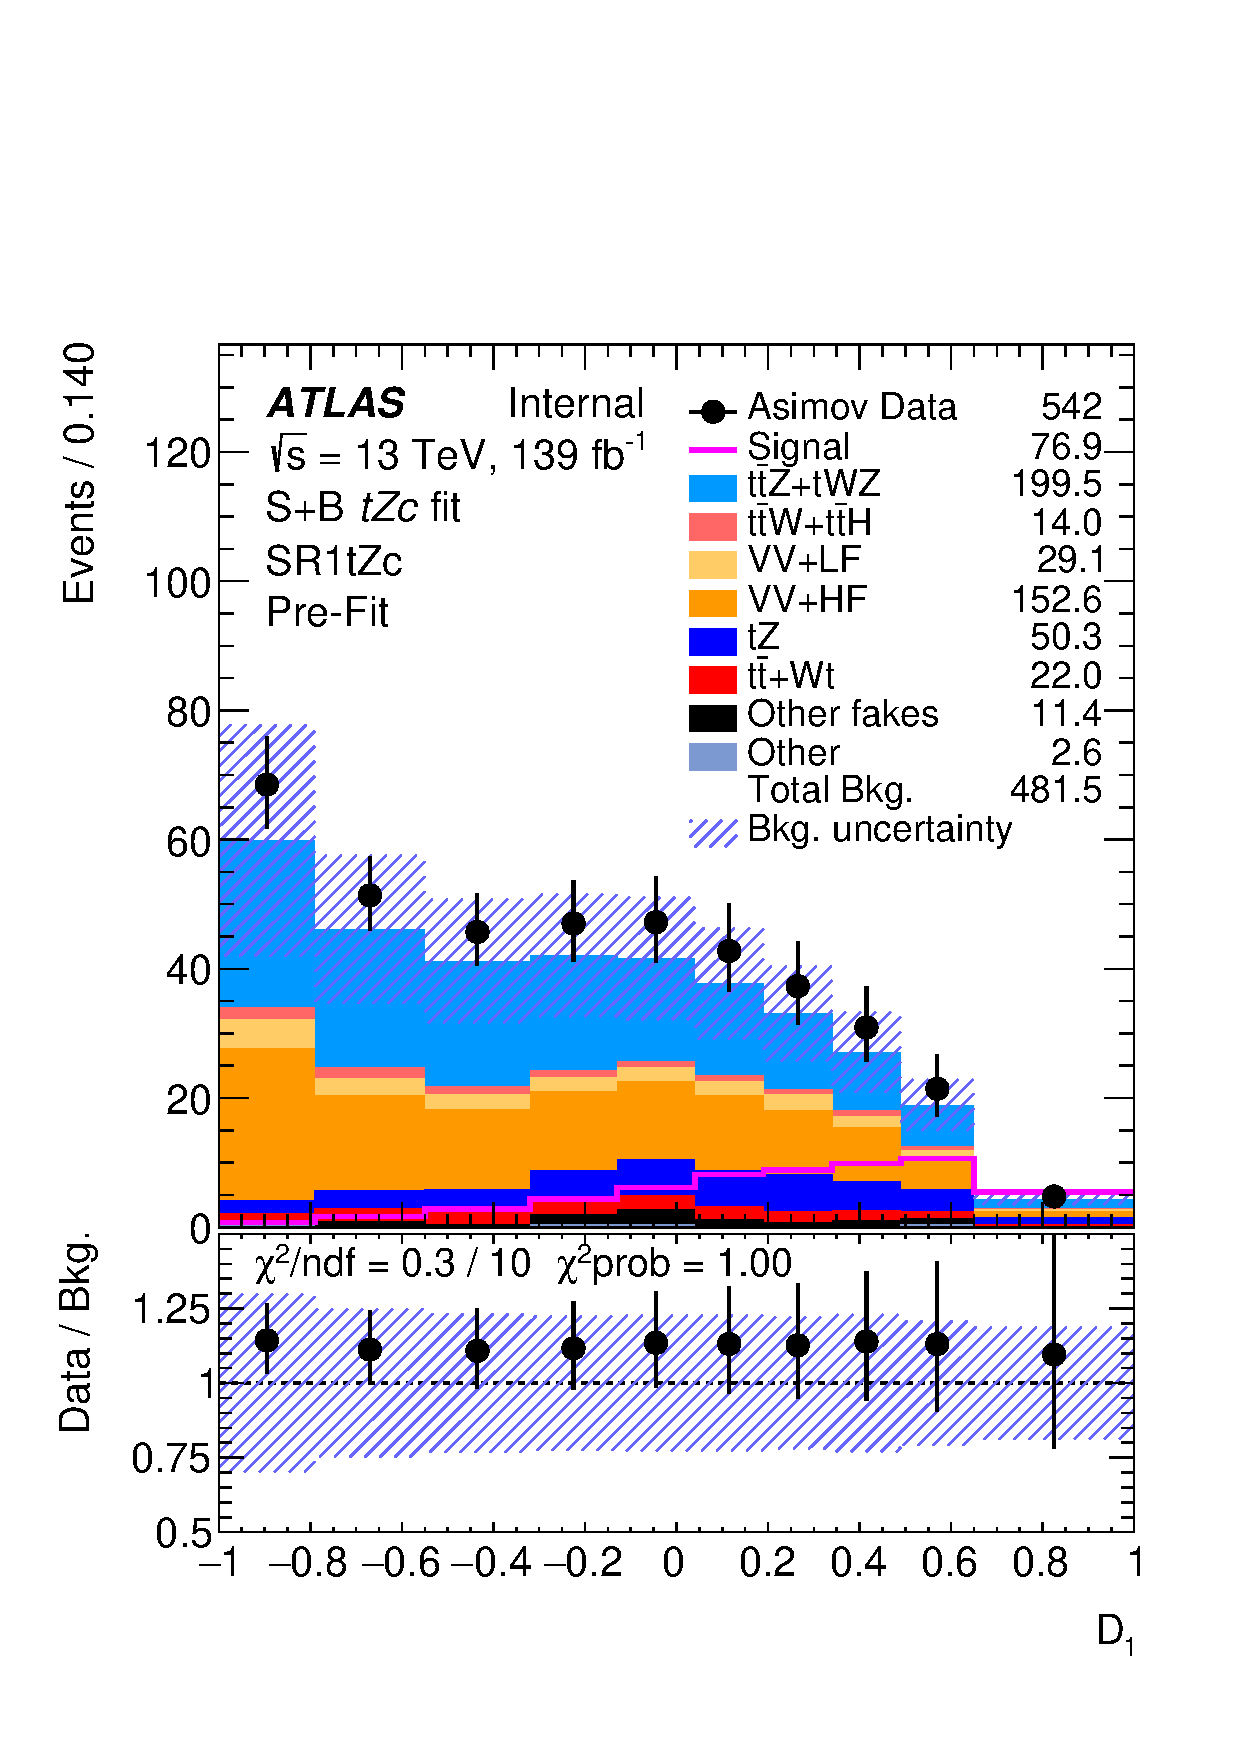
\includegraphics[width=.45\textwidth]{Appendices/AP8/figures/SPLUSB_CRSR_UsingSMTFullSys/Plots/SR1} &
		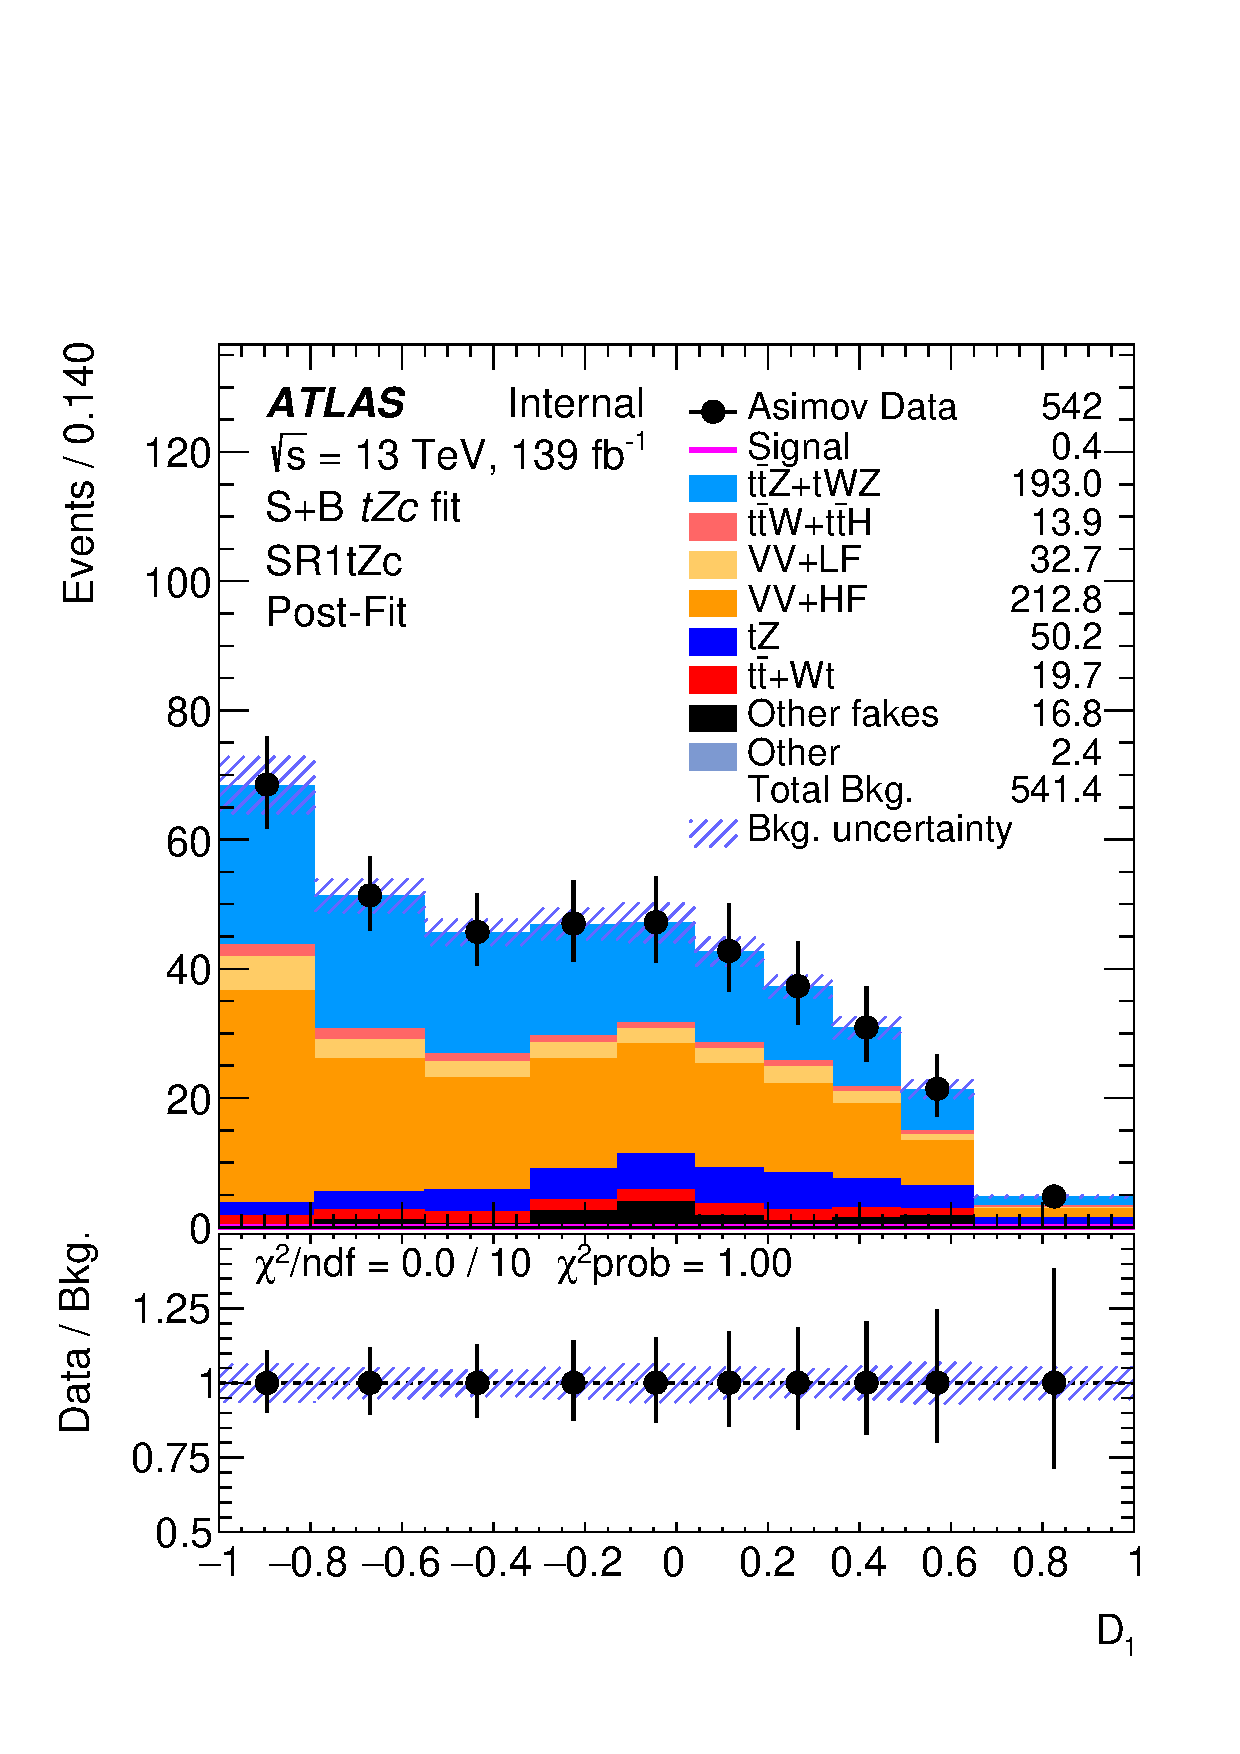
\includegraphics[width=.45\textwidth]{Appendices/AP8/figures/SPLUSB_CRSR_UsingSMTFullSys/Plots/SR1_postFit} \\
		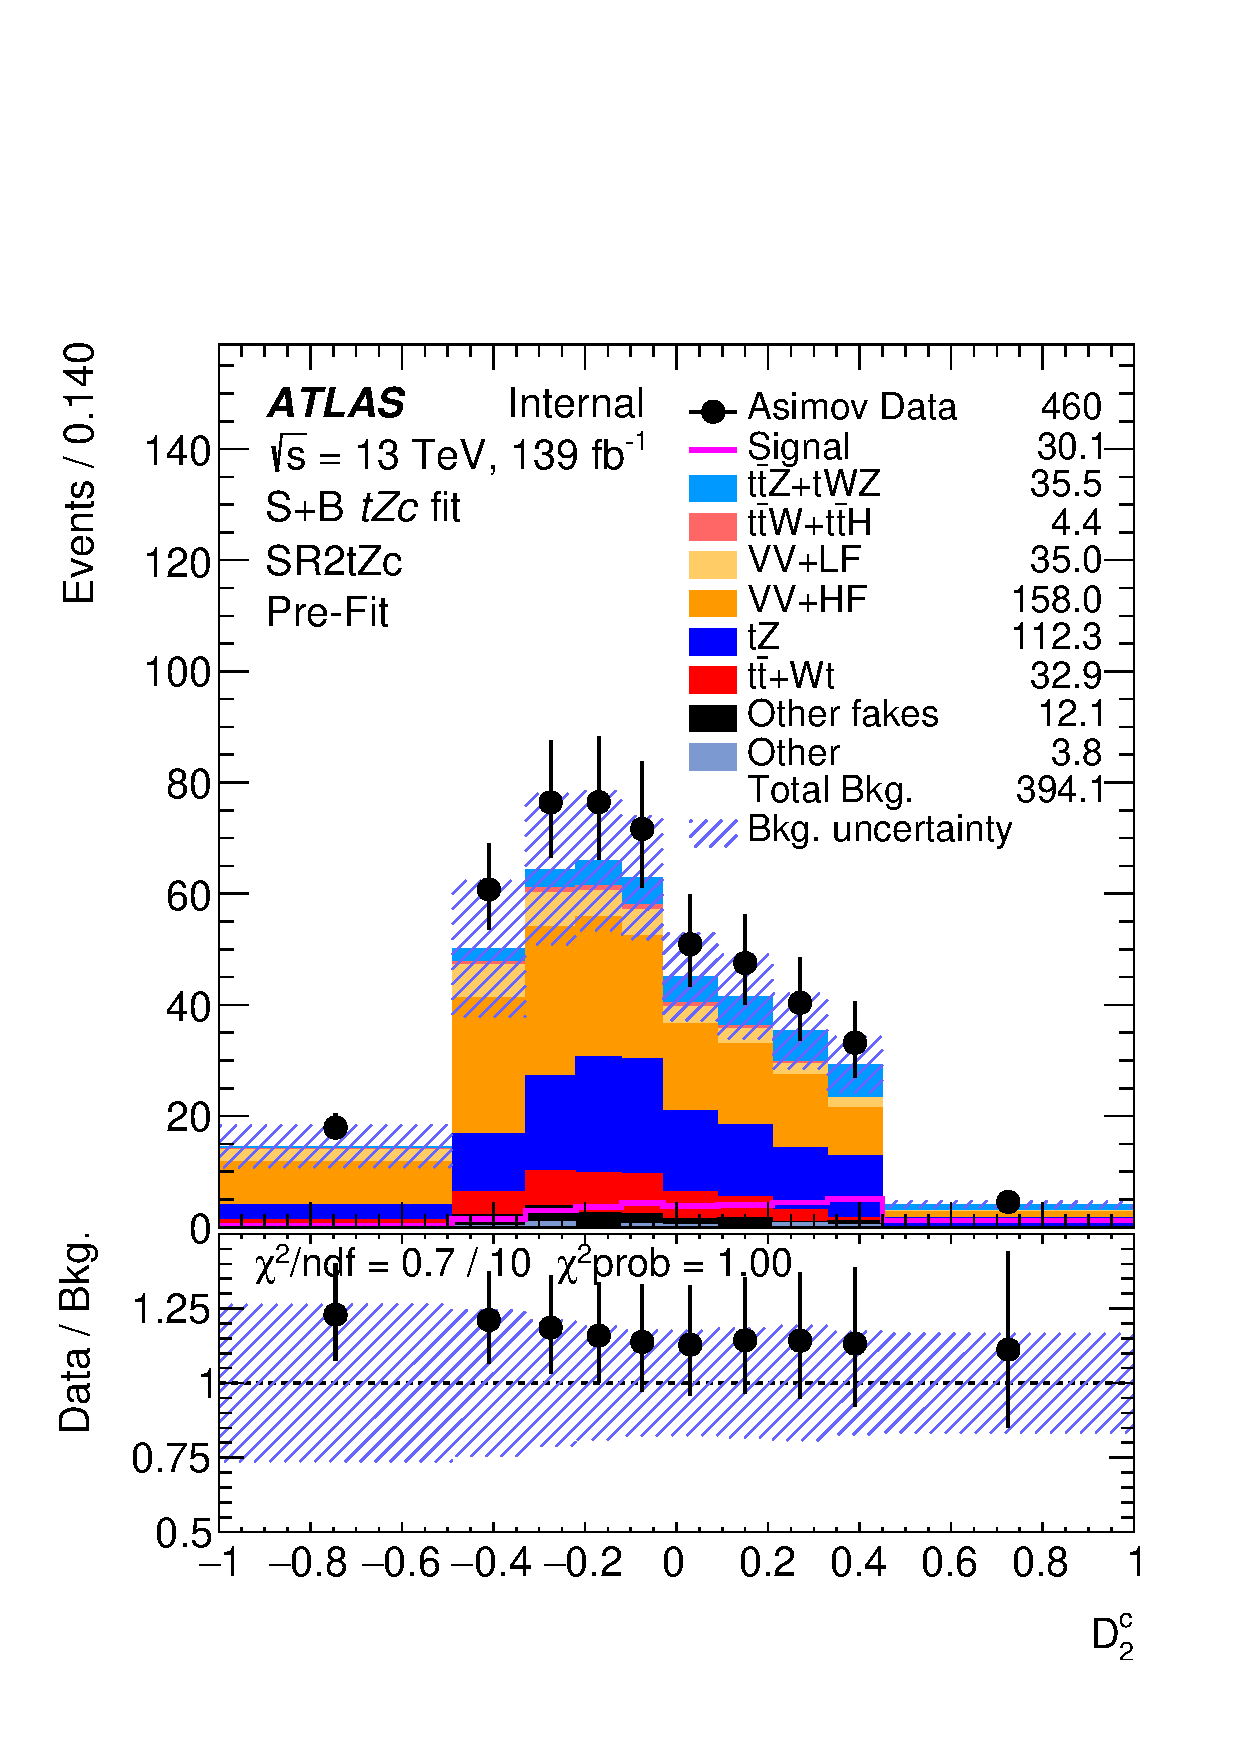
\includegraphics[width=.45\textwidth]{Appendices/AP8/figures/SPLUSB_CRSR_UsingSMTFullSys/Plots/SR2} &
		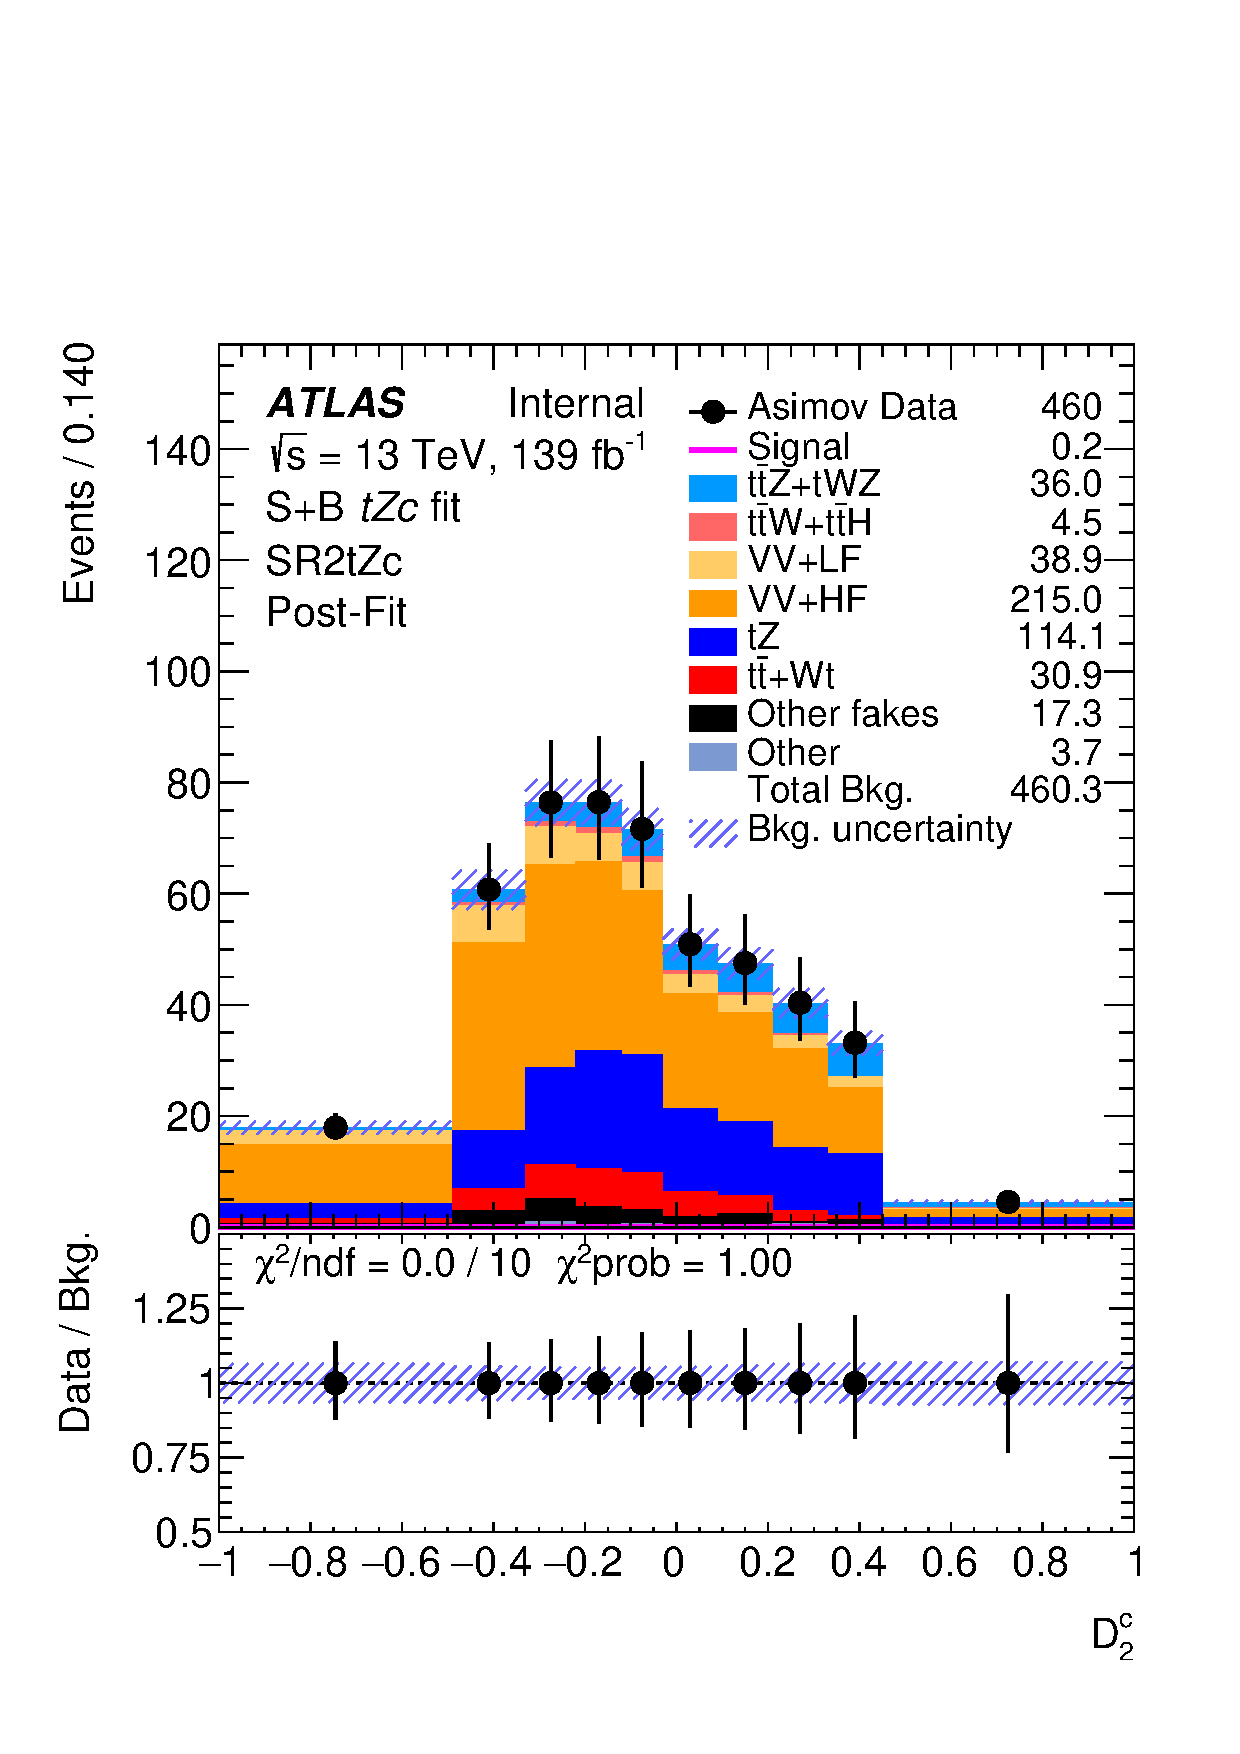
\includegraphics[width=.45\textwidth]{Appendices/AP8/figures/SPLUSB_CRSR_UsingSMTFullSys/Plots/SR2_postFit} \\
	\end{tabular}
	\caption{Pre-fit (left) and post-fit (right) BDTG output distributions in SR1 and SR2 for the S+B \tZc fit in SRs+CRs with realistic Asimov.
		\ErrStatSys
	}%
	\label{fig:stat_smt:tzc:splusb:crsr:srplots:1}
\end{figure}

\begin{figure}[htbp]
	\centering
	\begin{tabular}{cc}
		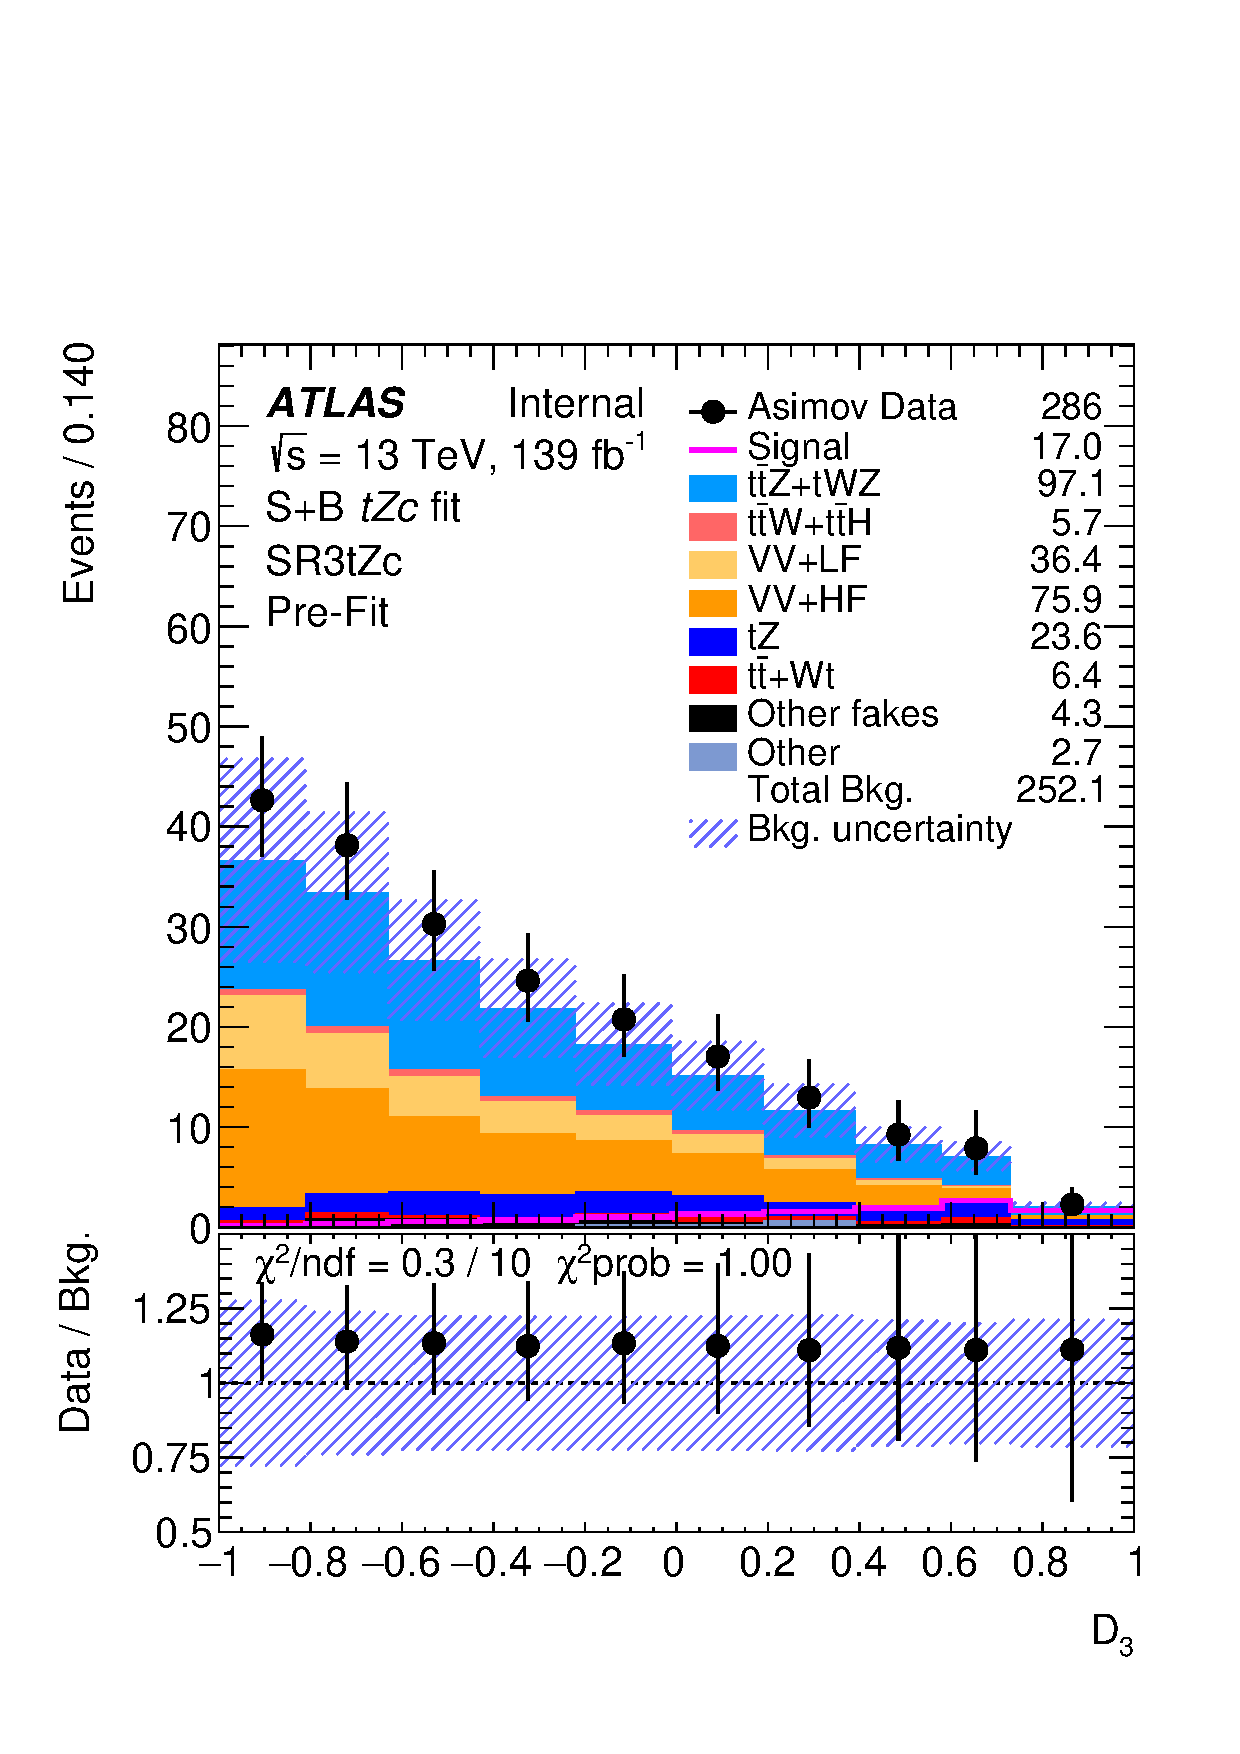
\includegraphics[width=.45\textwidth]{Appendices/AP8/figures/SPLUSB_CRSR_UsingSMTFullSys/Plots/SR3} &
		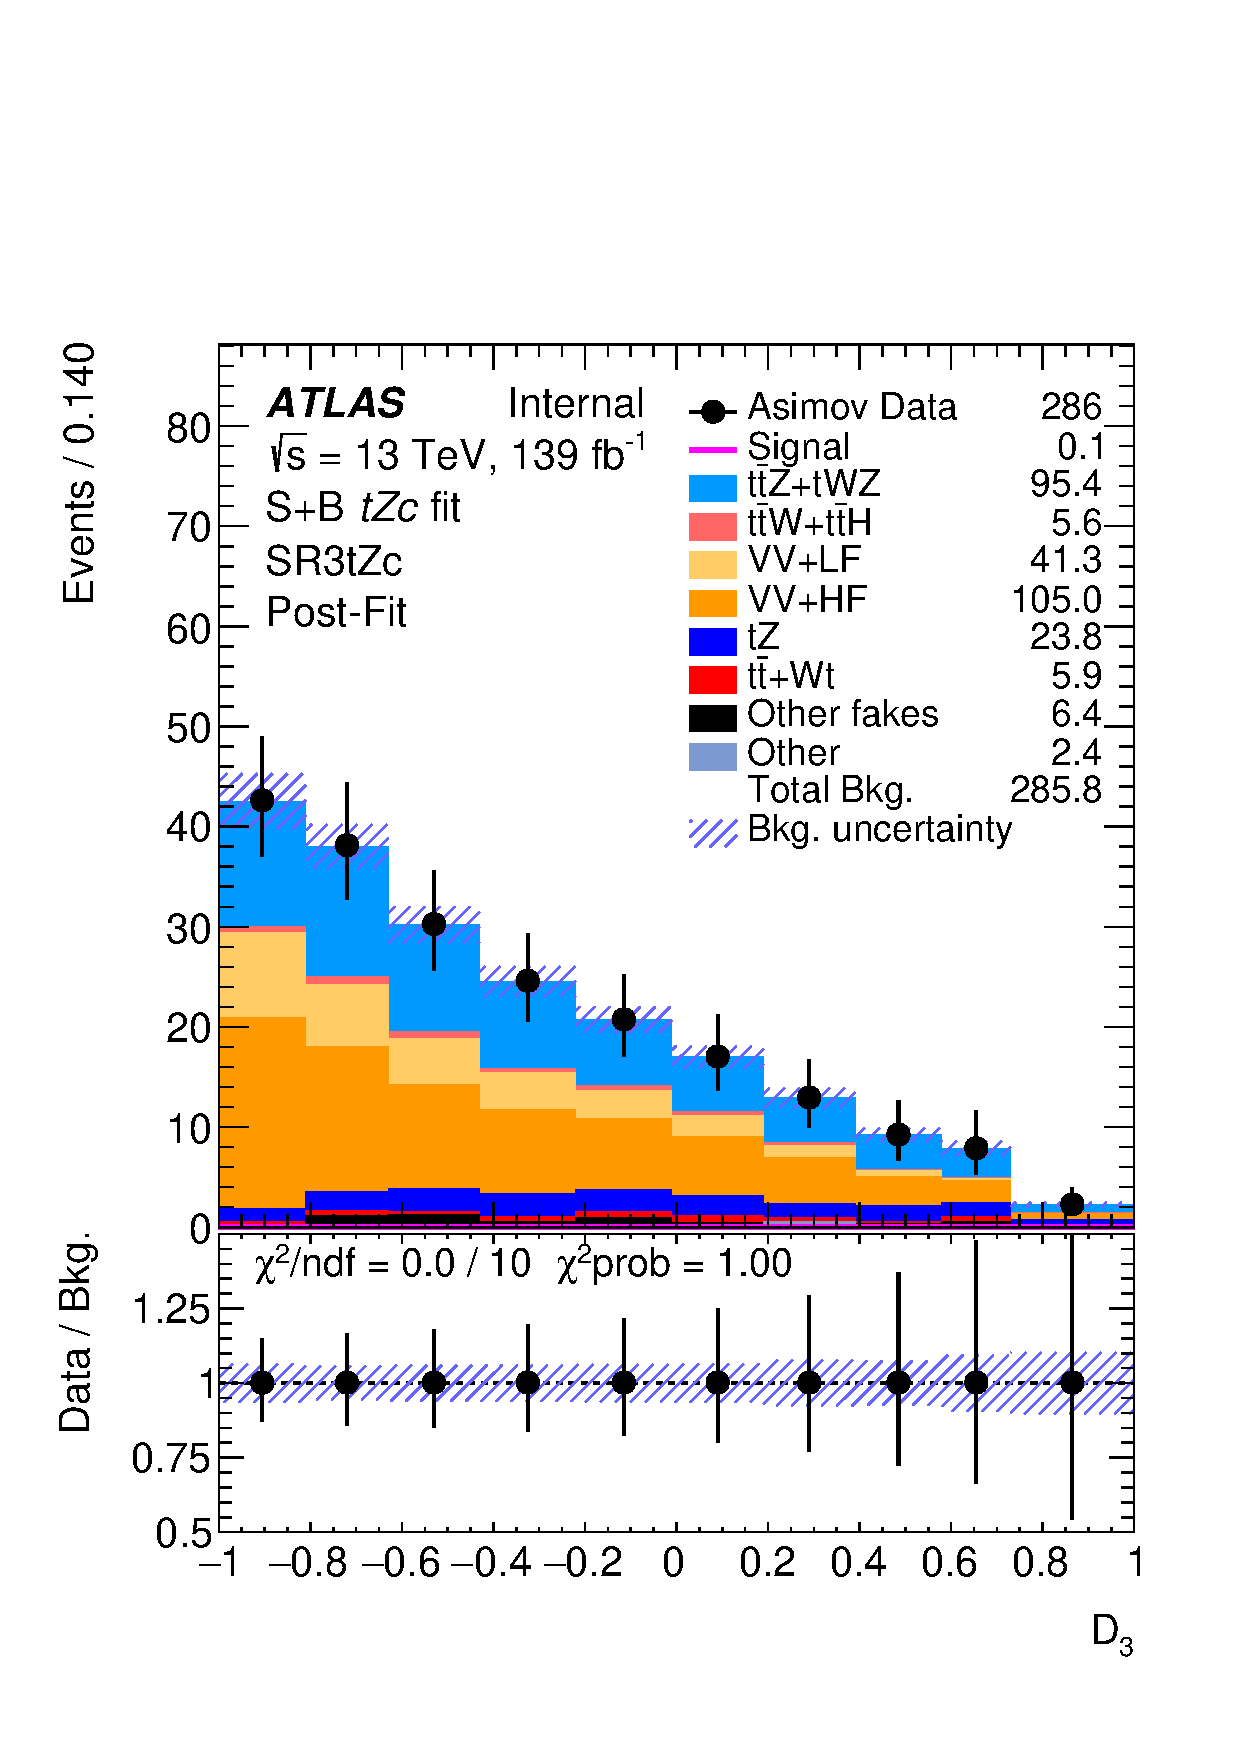
\includegraphics[width=.45\textwidth]{Appendices/AP8/figures/SPLUSB_CRSR_UsingSMTFullSys/Plots/SR3_postFit} \\
	\end{tabular}
	\caption{Pre-fit (left) and post-fit (right) leading lepton \pt distributions in SR3 for the S+B \tZc fit in SRs+CRs with realistic Asimov.
		\ErrStatSys
	}%
	\label{fig:stat_smt:tzc:splusb:crsr:srplots:2}
\end{figure}

\begin{figure}[htbp]
	\centering
	\begin{tabular}{cc}
		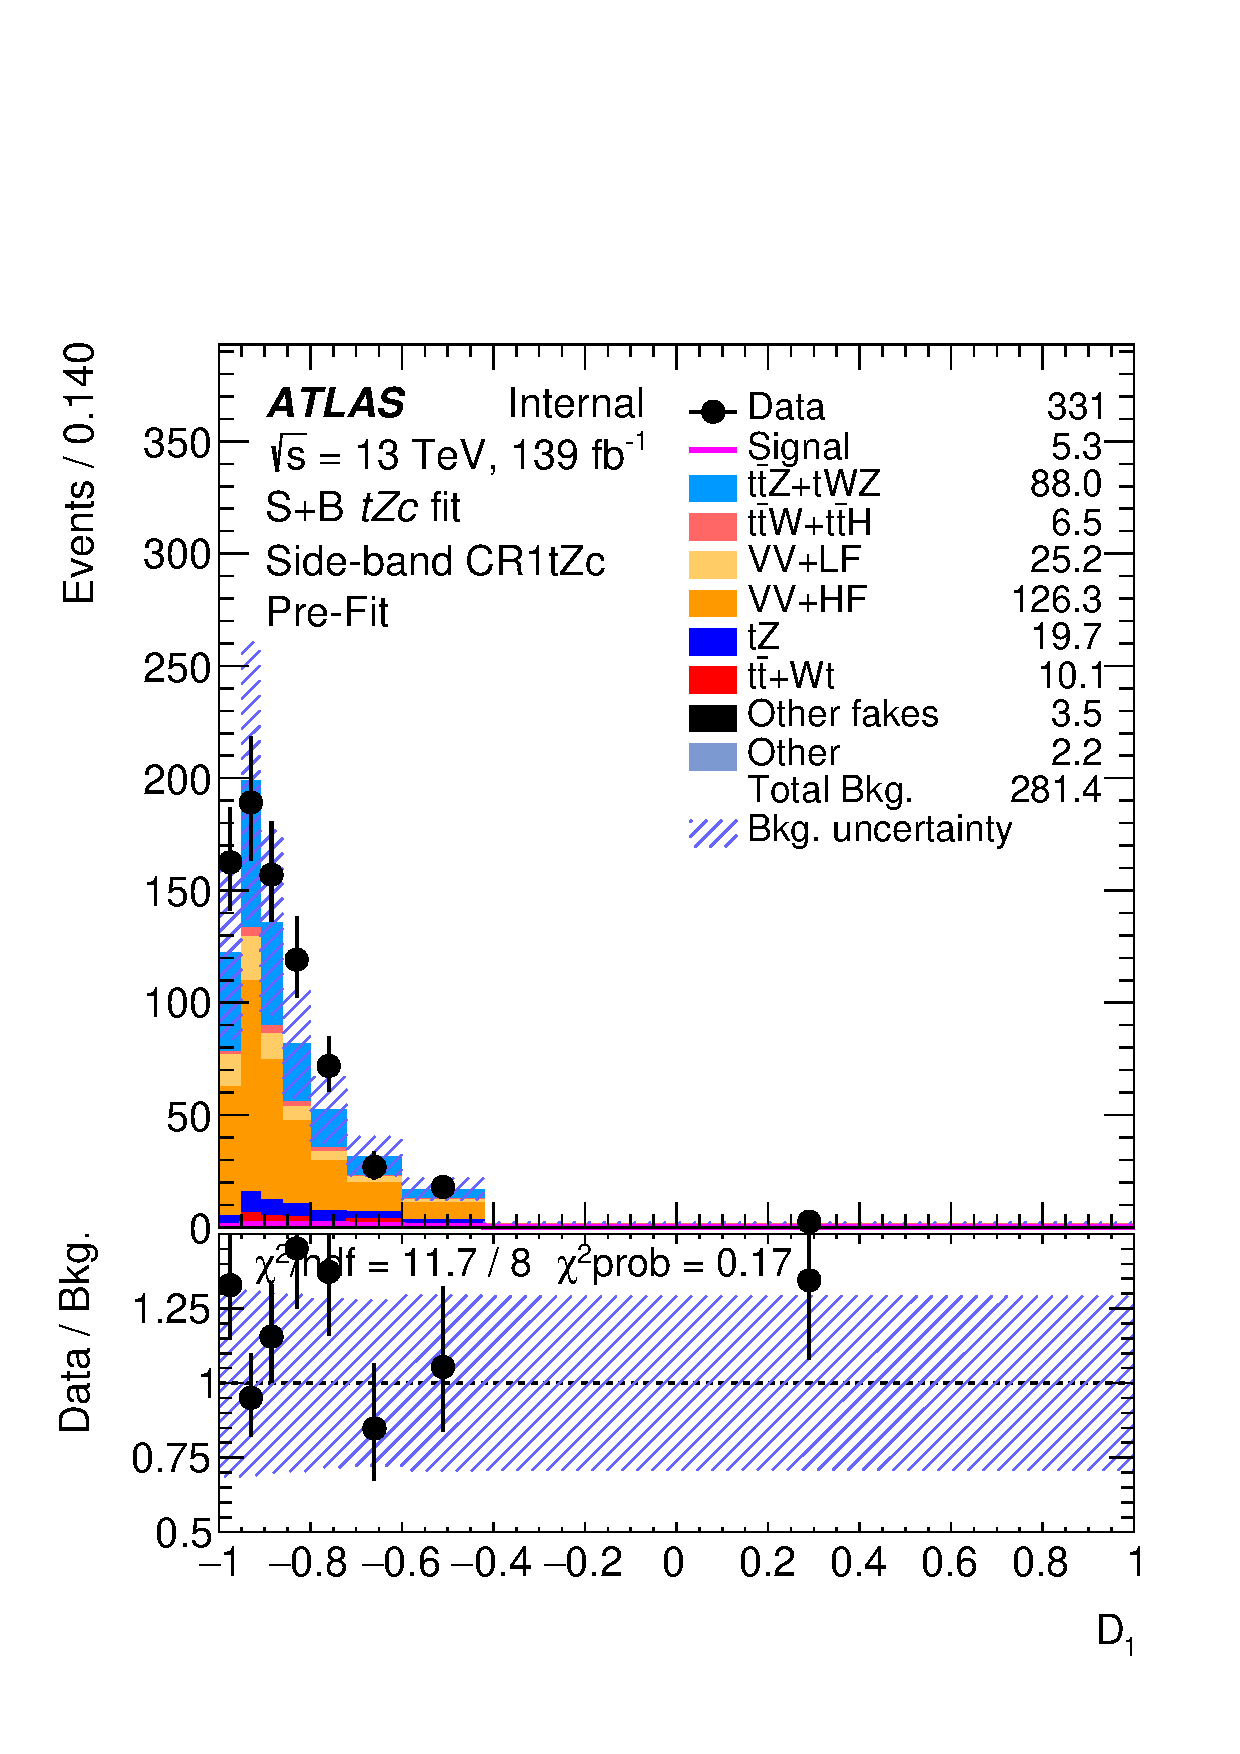
\includegraphics[width=.45\textwidth]{Appendices/AP8/figures/SPLUSB_CRSR_UsingSMTFullSys/Plots/SBCR1} &
		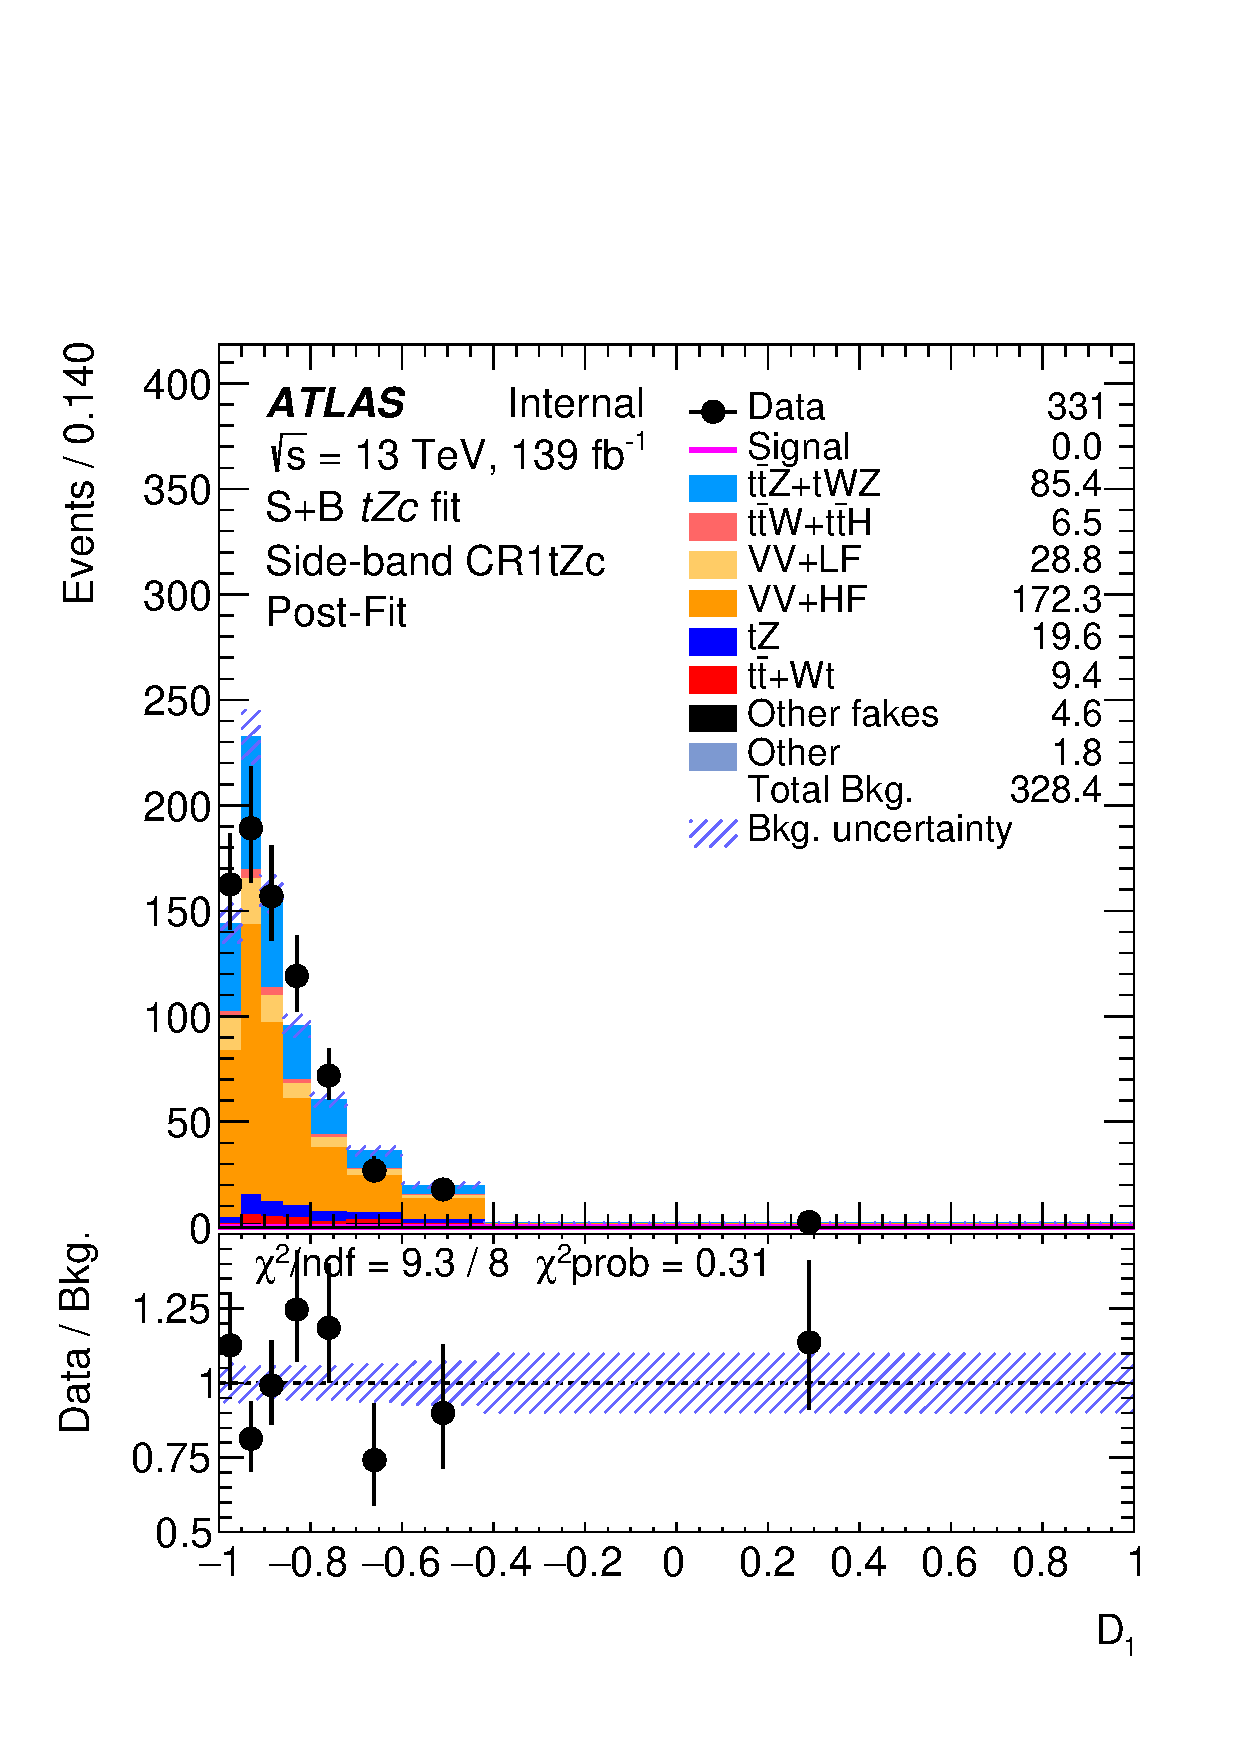
\includegraphics[width=.45\textwidth]{Appendices/AP8/figures/SPLUSB_CRSR_UsingSMTFullSys/Plots/SBCR1_postFit} \\
		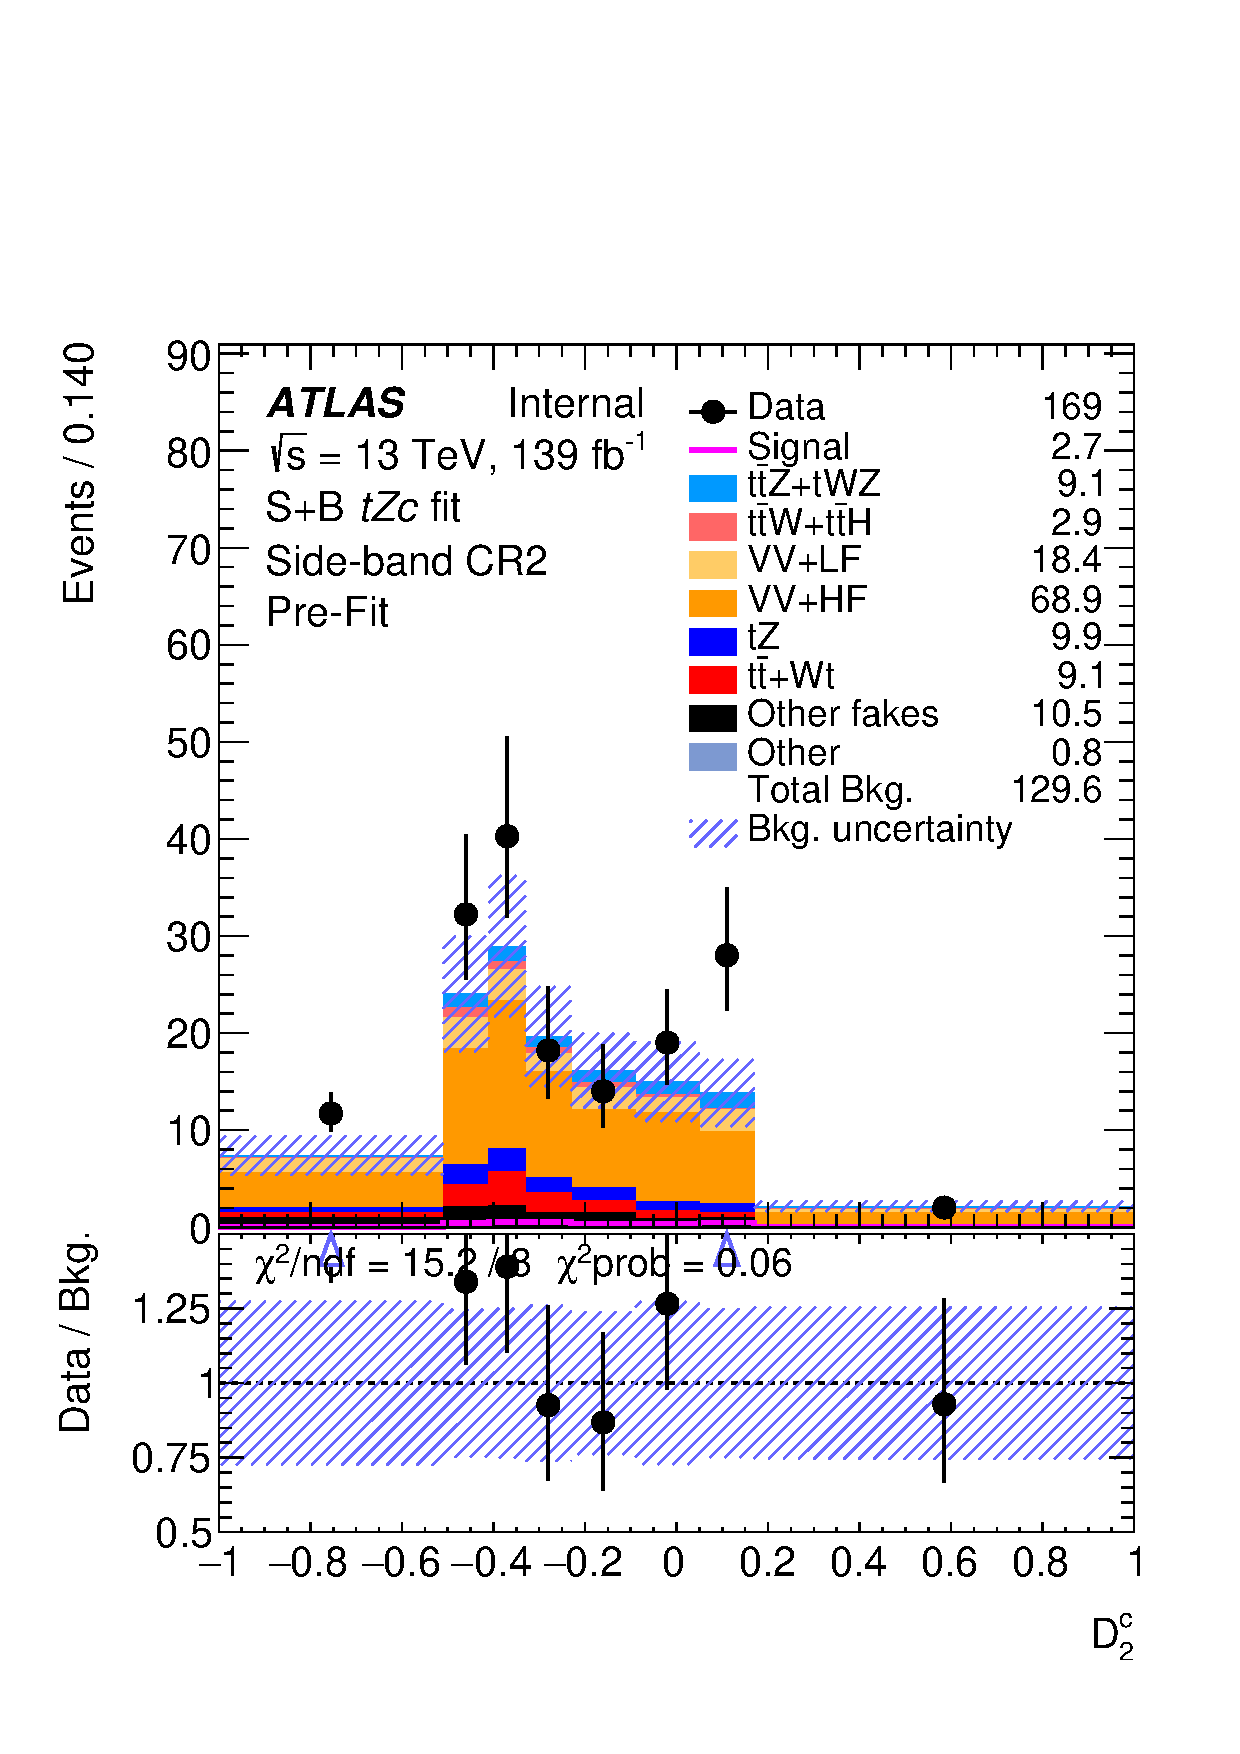
\includegraphics[width=.45\textwidth]{Appendices/AP8/figures/SPLUSB_CRSR_UsingSMTFullSys/Plots/SBCR2} &
		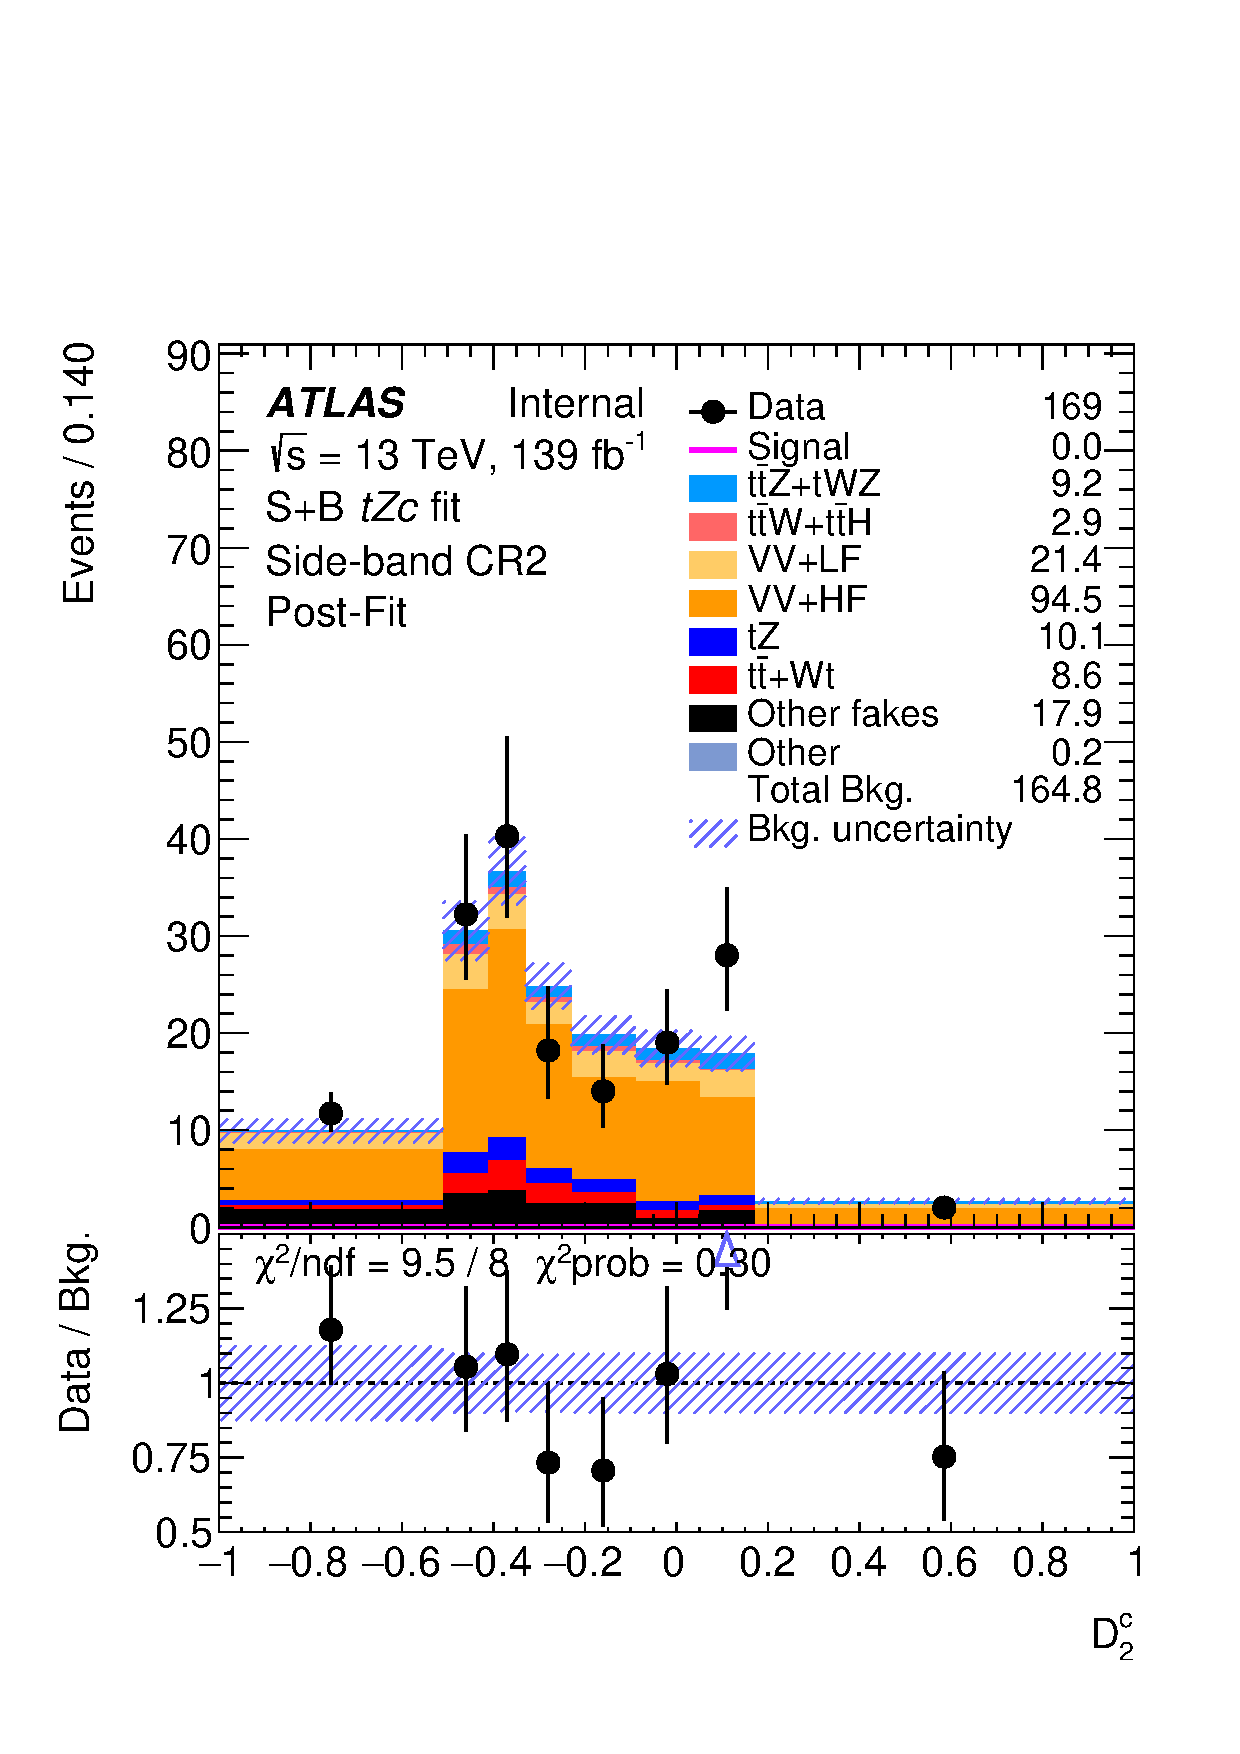
\includegraphics[width=.45\textwidth]{Appendices/AP8/figures/SPLUSB_CRSR_UsingSMTFullSys/Plots/SBCR2_postFit} \\
	\end{tabular}
	\caption{Pre-fit (left) and post-fit (right) BDTG output distributions in the side-band CRs for the S+B \tZc fit in SRs+CRs with realistic Asimov.
		\ErrStatSys
	}%
	\label{fig:stat_smt:tzc:splusb:crsr:crplots:1}
\end{figure}

\begin{figure}[htbp]
	\centering
	\begin{tabular}{cc}
		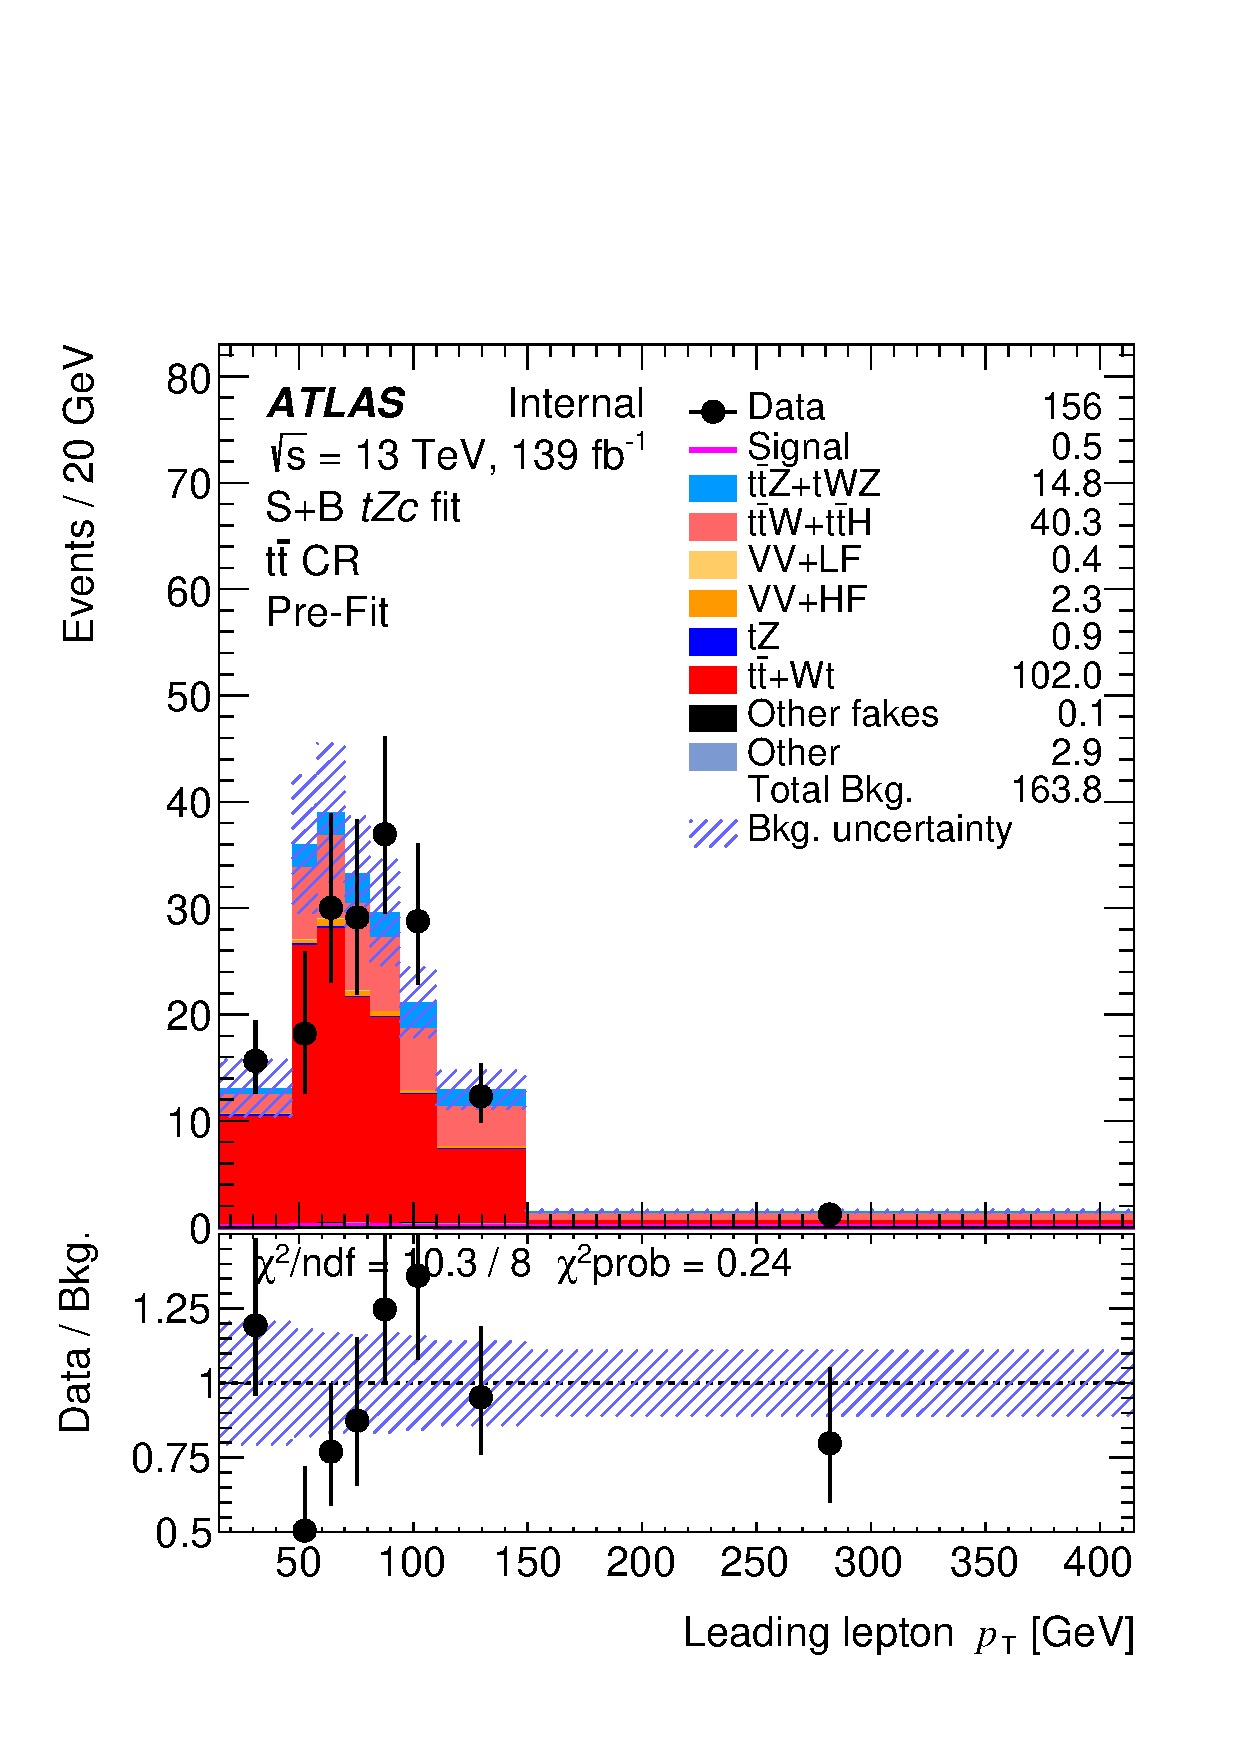
\includegraphics[width=.45\textwidth]{Appendices/AP8/figures/SPLUSB_CRSR_UsingSMTFullSys/Plots/TTCR} &
		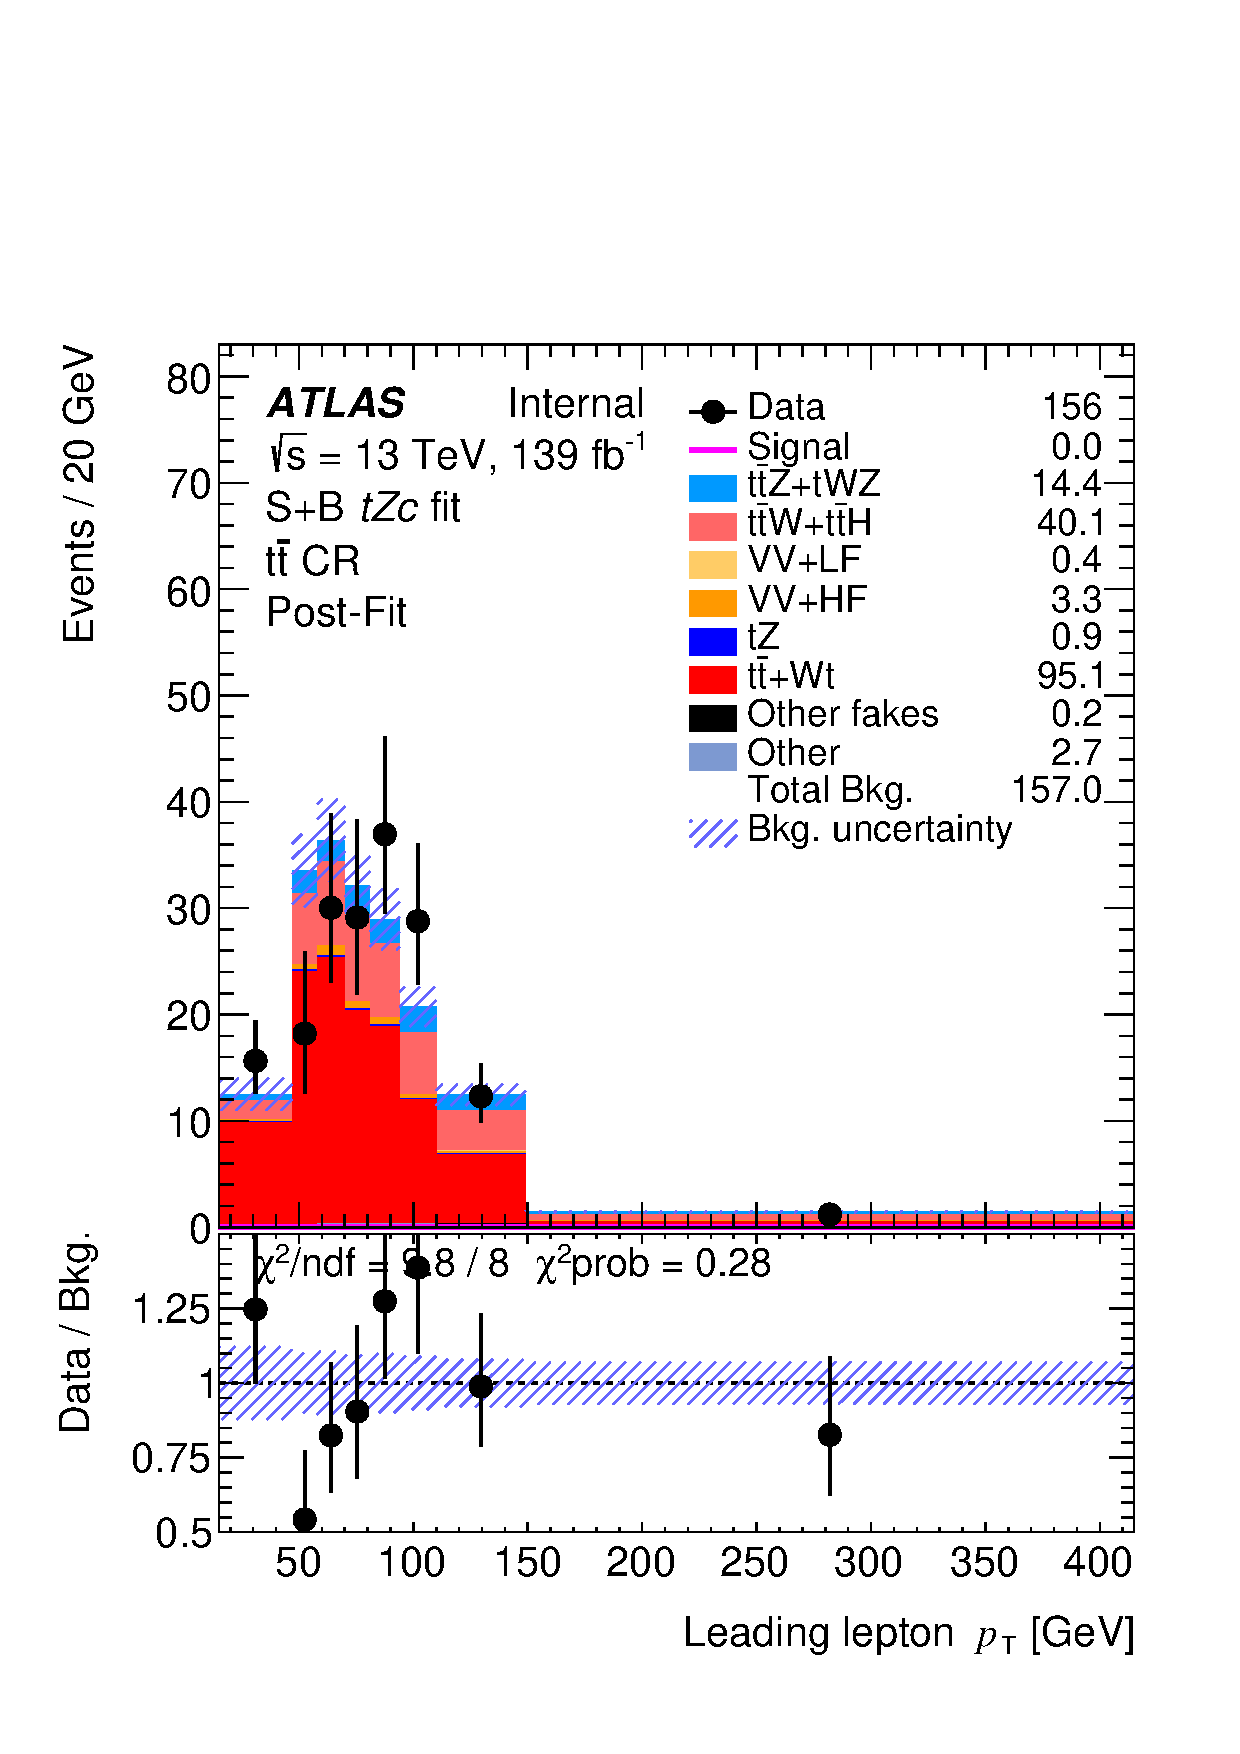
\includegraphics[width=.45\textwidth]{Appendices/AP8/figures/SPLUSB_CRSR_UsingSMTFullSys/Plots/TTCR_postFit} \\
		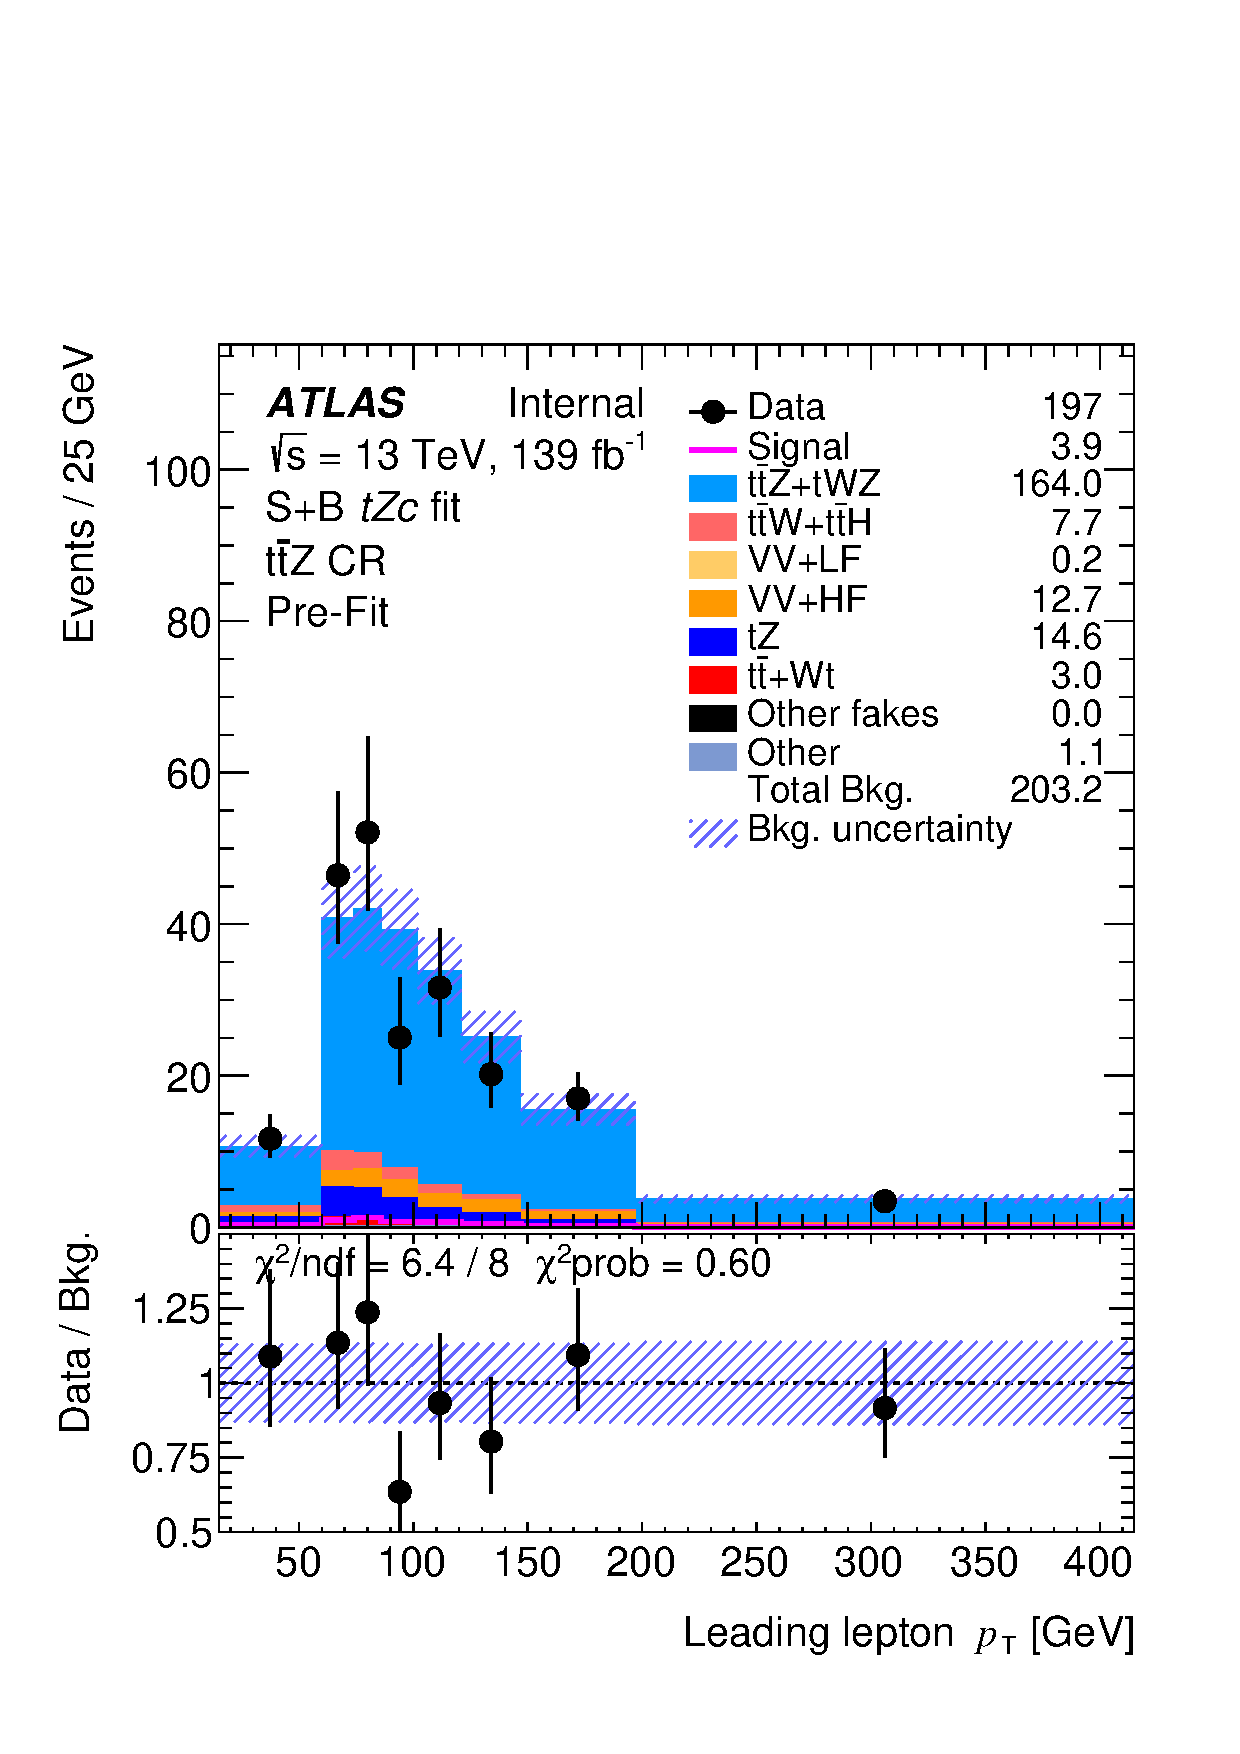
\includegraphics[width=.45\textwidth]{Appendices/AP8/figures/SPLUSB_CRSR_UsingSMTFullSys/Plots/TTZCR} &
		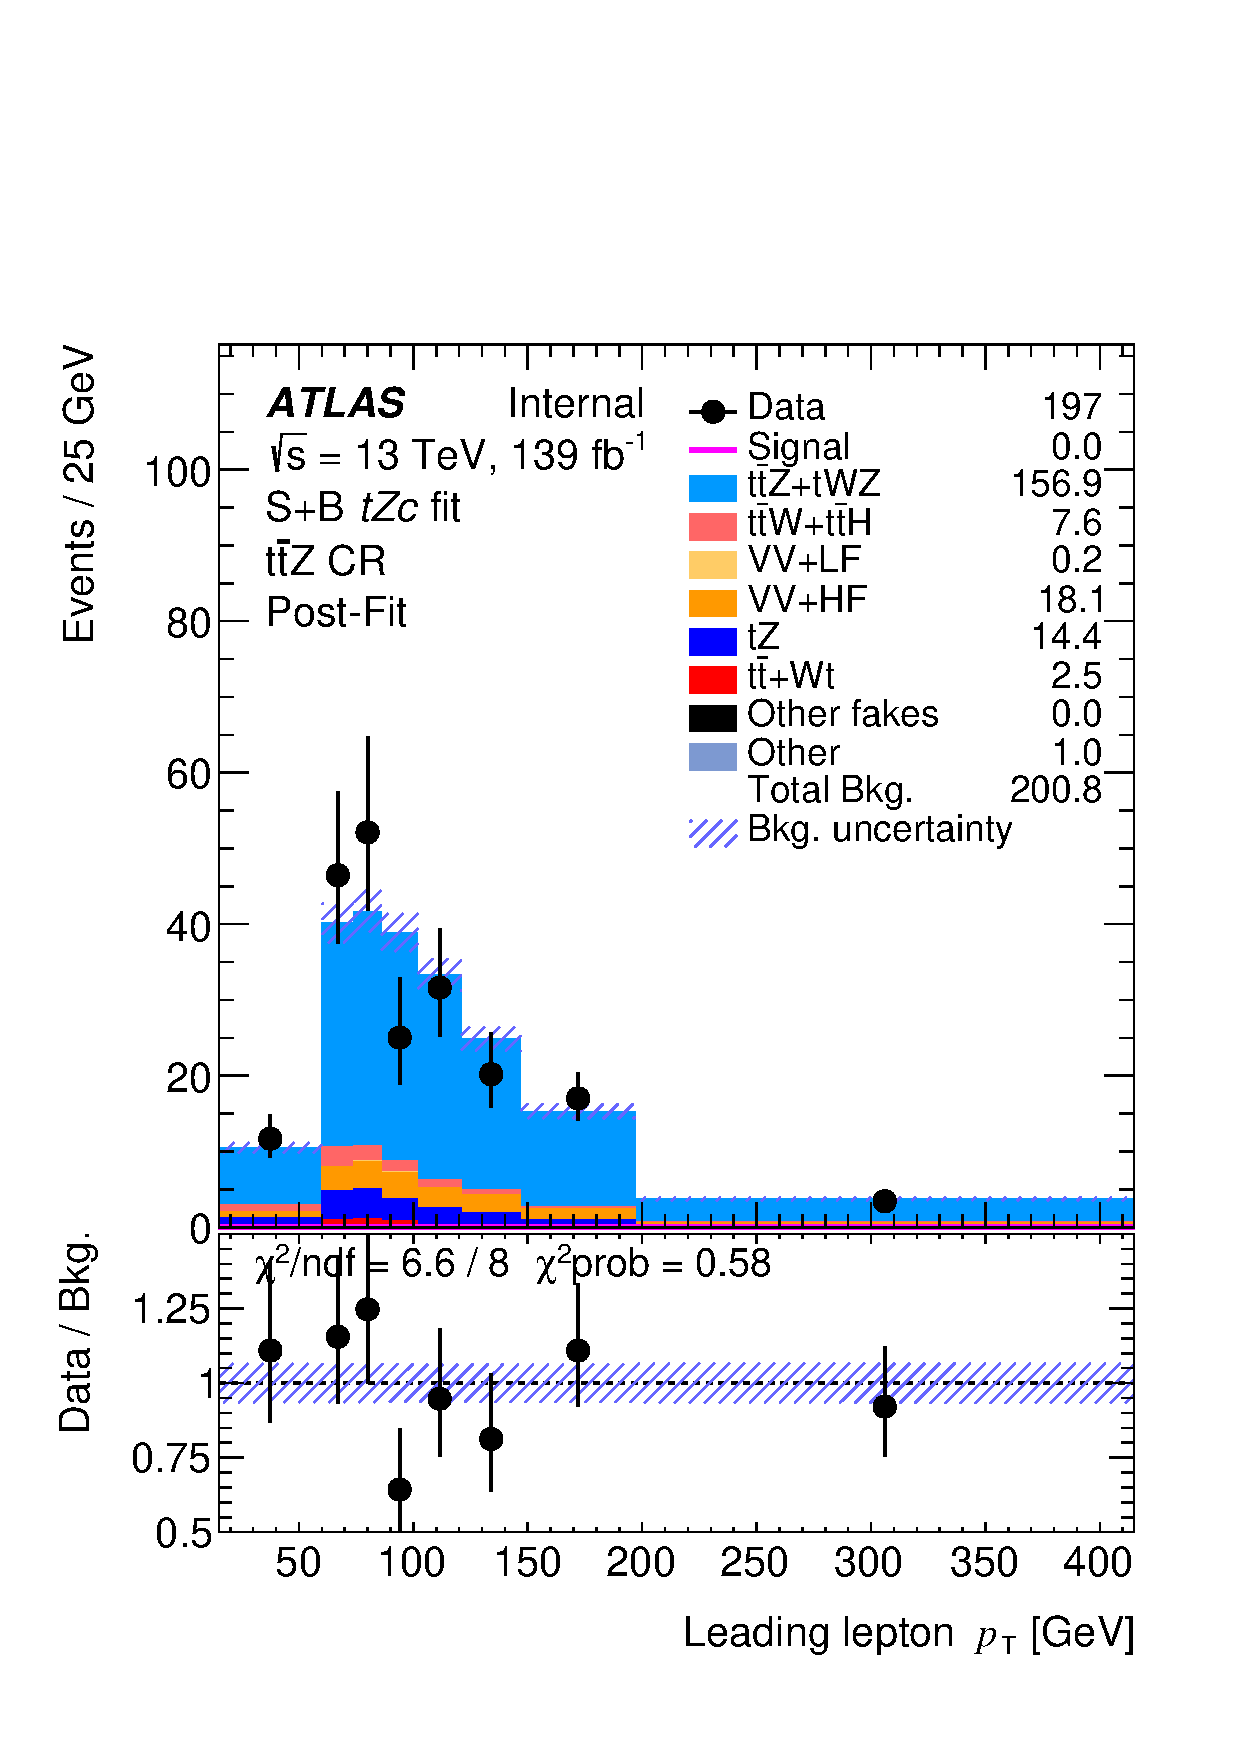
\includegraphics[width=.45\textwidth]{Appendices/AP8/figures/SPLUSB_CRSR_UsingSMTFullSys/Plots/TTZCR_postFit} \\
	\end{tabular}
	\caption{Pre-fit (left) and post-fit (right) leading lepton \pt distributions in the \ttbar and \ttZ CRs for the S+B \tZc fit in SRs+CRs with realistic Asimov.
		\ErrStatSys
	}%
	\label{fig:stat_smt:tzc:splusb:crsr:crplots:2}
\end{figure}

\FloatBarrier
The expected limits, together
with statistical only limits and the expected limits from the previous ATLAS
analysis~\cite{TOPQ-2017-06}, are reported in \Cref{tab:results:limits_smt}.\\
The overall impact of systematics on the expected limit is 24\%.\\
The limit from the previous analysis is improved by a factor of 3.1 for the \tZc coupling.
\begin{table}[htbp]
	\centering
	\begin{tabular}{lccc}
		\toprule
		\textbf{Limits} & \textbf{$-1\sigma$} & \textbf{Expected} & \textbf{$+1\sigma$} \\
		\midrule
		BR $\Pqt\rightarrow\PZ\Pqc$ \cite{TOPQ-2017-06} & \SI{2.2e-4}{} & \SI{3.2e-4}{} & \SI{4.6e-4}{} \\
		BR $\Pqt\rightarrow\PZ\Pqc$  (stat. only)                 & \SI{5.7e-5}{} & \SI{7.9e-5}{} & \SI{10.9e-5}{} \\
		BR $\Pqt\rightarrow\PZ\Pqc$                                    & \SI{7.4e-5}{} & \SI{10.4e-5}{} & \SI{14.8e-5}{} \\		 % SMT limits minus =7.44e-05, expected=10.32, plus=14.78
		\bottomrule
	\end{tabular}
	\caption{
		Expected limits on the branching ratios of $\Pqt\rightarrow\PZ\Pqc$ using SMT.
		Expected limit from \cite{TOPQ-2017-06} is also included for reference.
	}%
	\label{tab:results:limits_smt}
\end{table}

